\chapter{結果}
\label{chap:results}

\subsection{ラベルノイズ付与による変化}
$\sigma$別に,それぞれのラベルノイズにおける詳細なエラー率を図\ref{fig:errors_by_label_noise_variance_0},図\ref{fig:coloredeminst_1000},図\ref{fig:errors_by_label_noise_variance_3612}
図\ref{fig:coloredeminst_10000}にそれぞれ示す.
特に$\gamma$が付与されている結果において,3つのフェーズに分けることができる.
\begin{itemize}
    \item Phase1 : テストエラー率と訓練エラー率がともに低下する.
    \item Phase2 : 訓練エラー率は引き続き低下するが,テストエラー率は上昇に転じる.
    \item Phase3 : 訓練エラー率はさらに低下するが,テストエラー率の上昇は緩やかになる.
\end{itemize}
色と数字の学習に関して,色よりも数字のほうが訓練・テストエラー率が高いことから,数字よりも色の難易度が低く,学習しやすいことが確認できる.
5層のCNNに関して,Phase1では,中段の結果を見ると興味深いことに,Colorの誤り率が50\% あたりで低下が停止し,Digitの精度向上を待っているような学習曲線を確認できる.
そして,どちらも50\% の訓練データに対する,誤り率が到達した後に,さらに低下を同時に始める.また,Phase2,3 においては,訓練データに対する誤り率をラベルノイズあり・
なしで分けた結果を確認すると,ラベルノイズなしの誤り率で二重降下現象のような挙動を確認できる.ラベルノイズありに対する誤り率とテストデータに対する誤り率はPhase2,3において,
低下し続けている.これらの低下に関しては,8層のCNNでも同じような挙動を示している.
また,このラベルノイズに対する挙動は,Nakkiranの二重降下現象を確認した設定でも確認した.その結果を図\ref{fig:errors_by_label_noise_variance_0},図\ref{fig:errors_by_label_noise_variance_1000},
\begin{figure}[H]
    \centering
    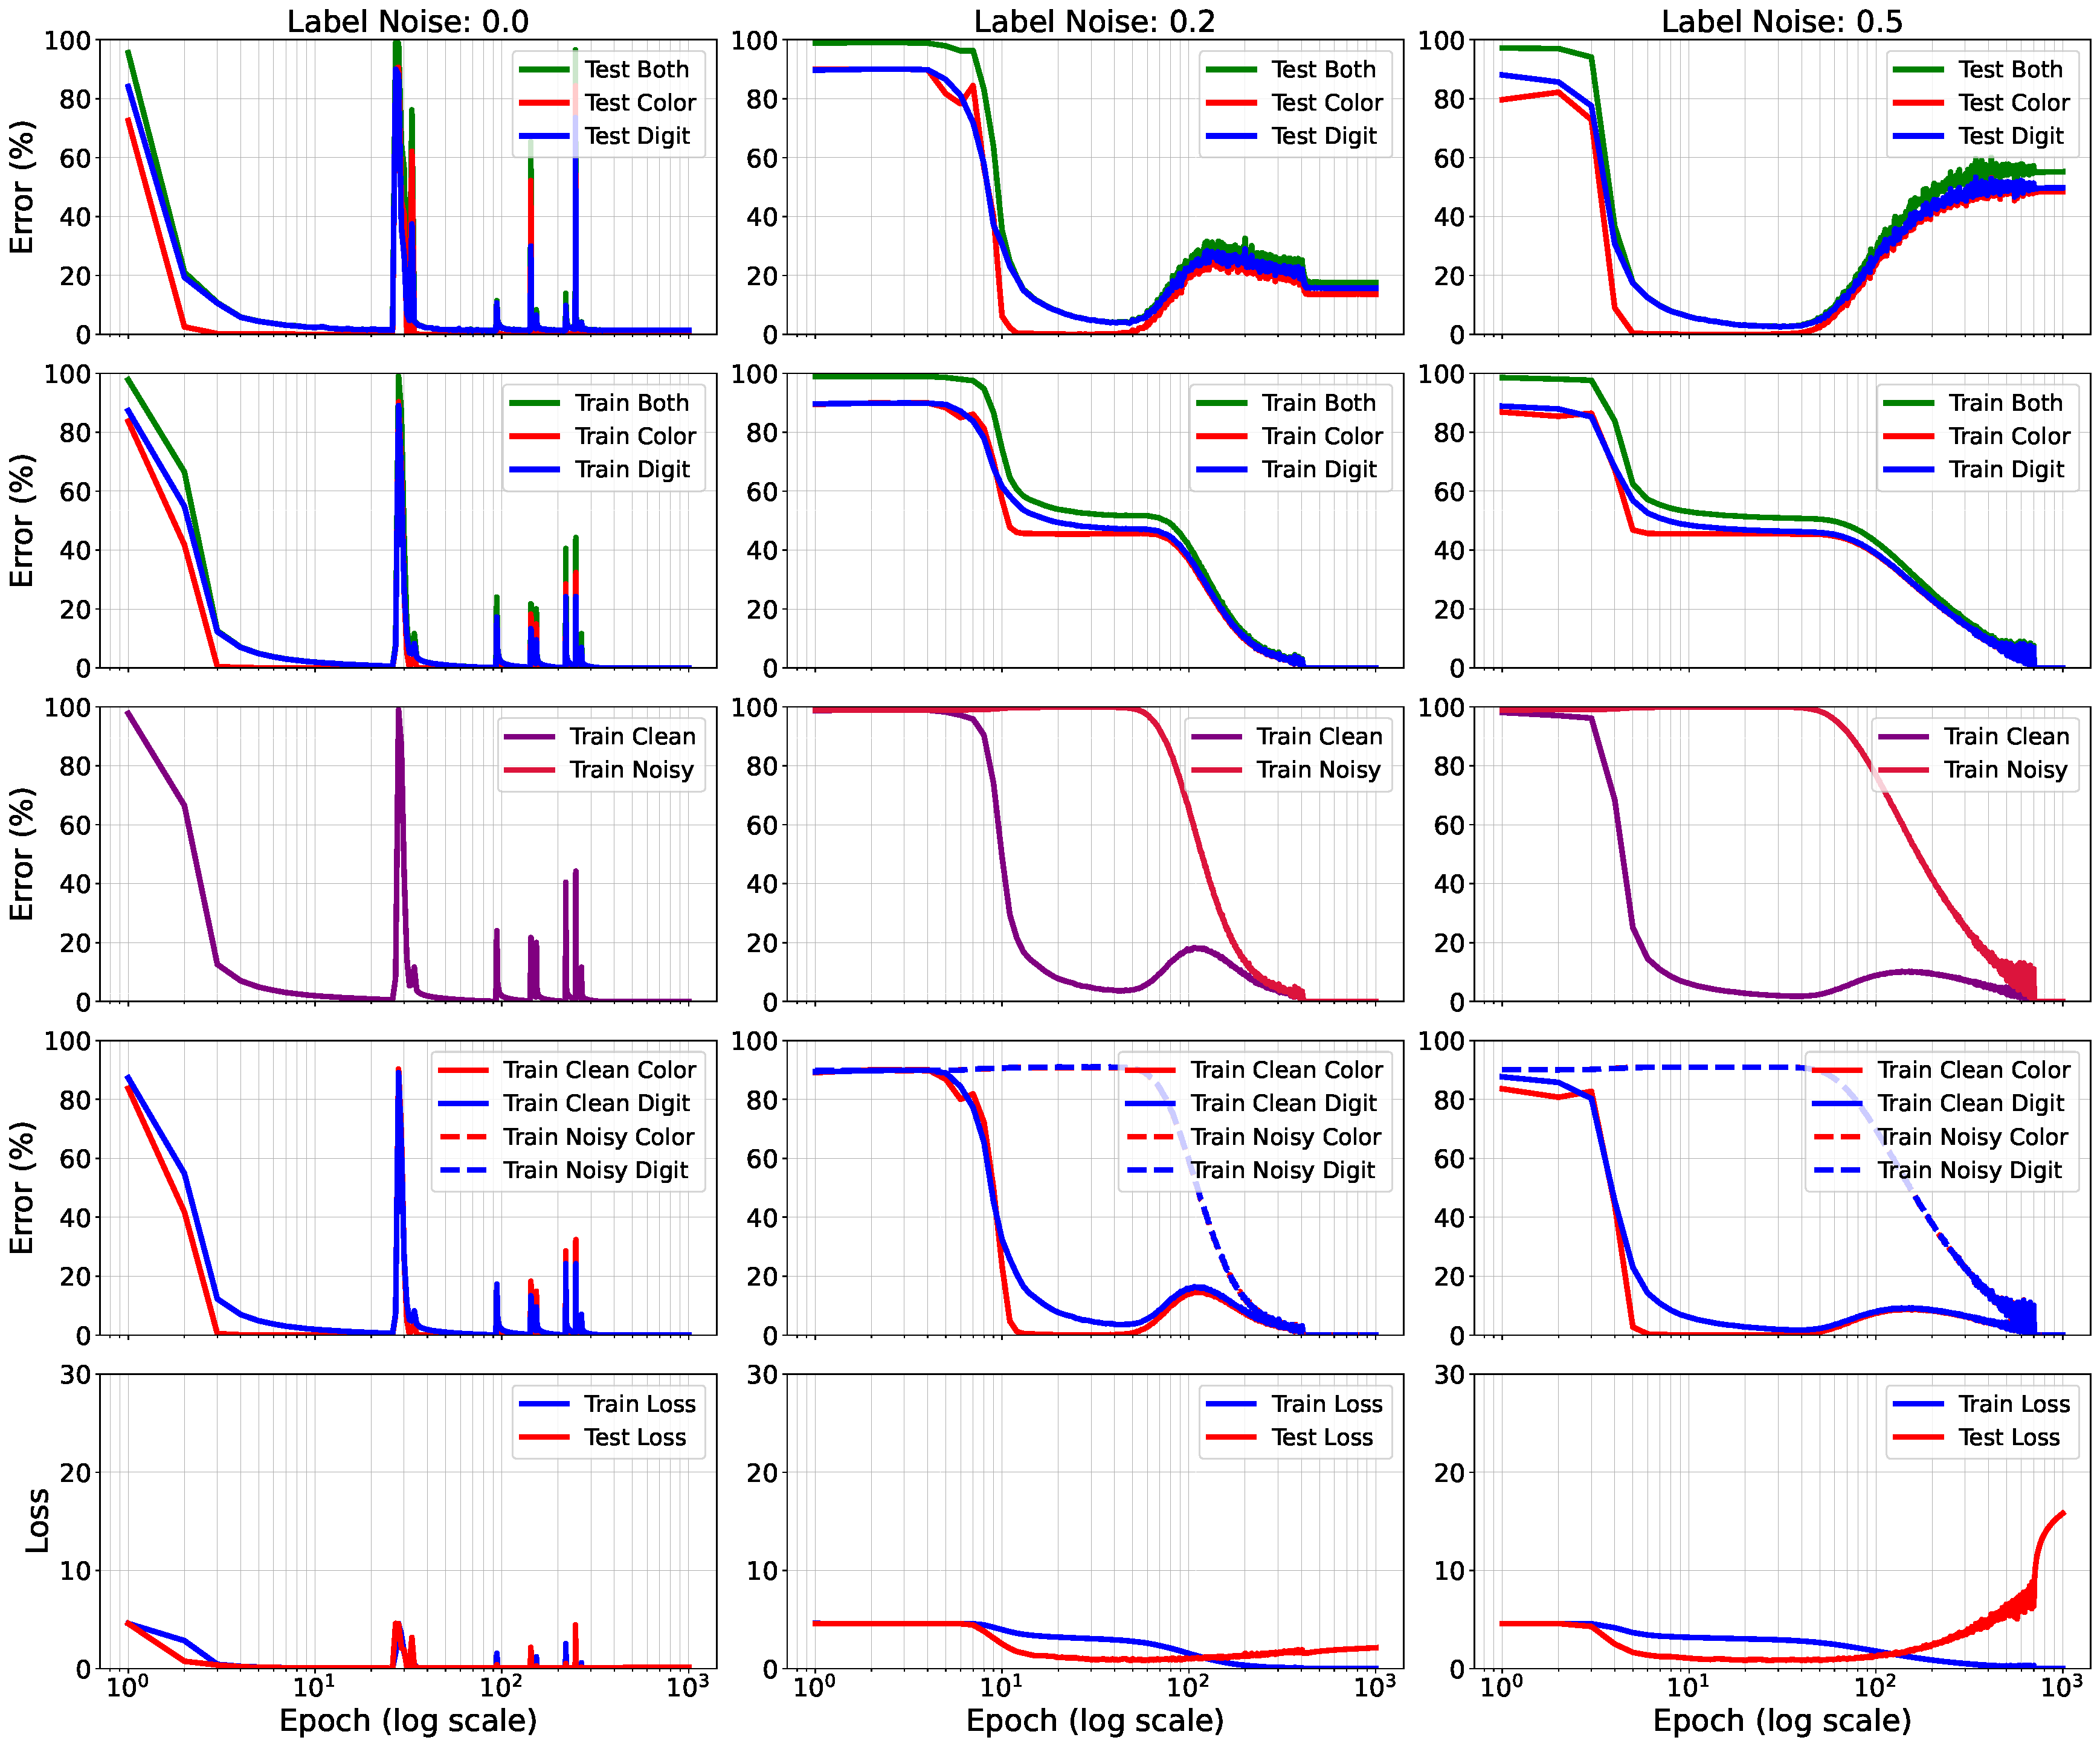
\includegraphics[width=\linewidth]{fig/erroe_metrics_by_variances/error_metrics_by_label_noise_variance_0.pdf}
    \caption{$\sigma^2 = 0$のときのそれぞれのラベルノイズにおける結果}
    \label{fig:errors_by_label_noise_variance_0}
\end{figure}

\begin{figure}[H]
    \centering
    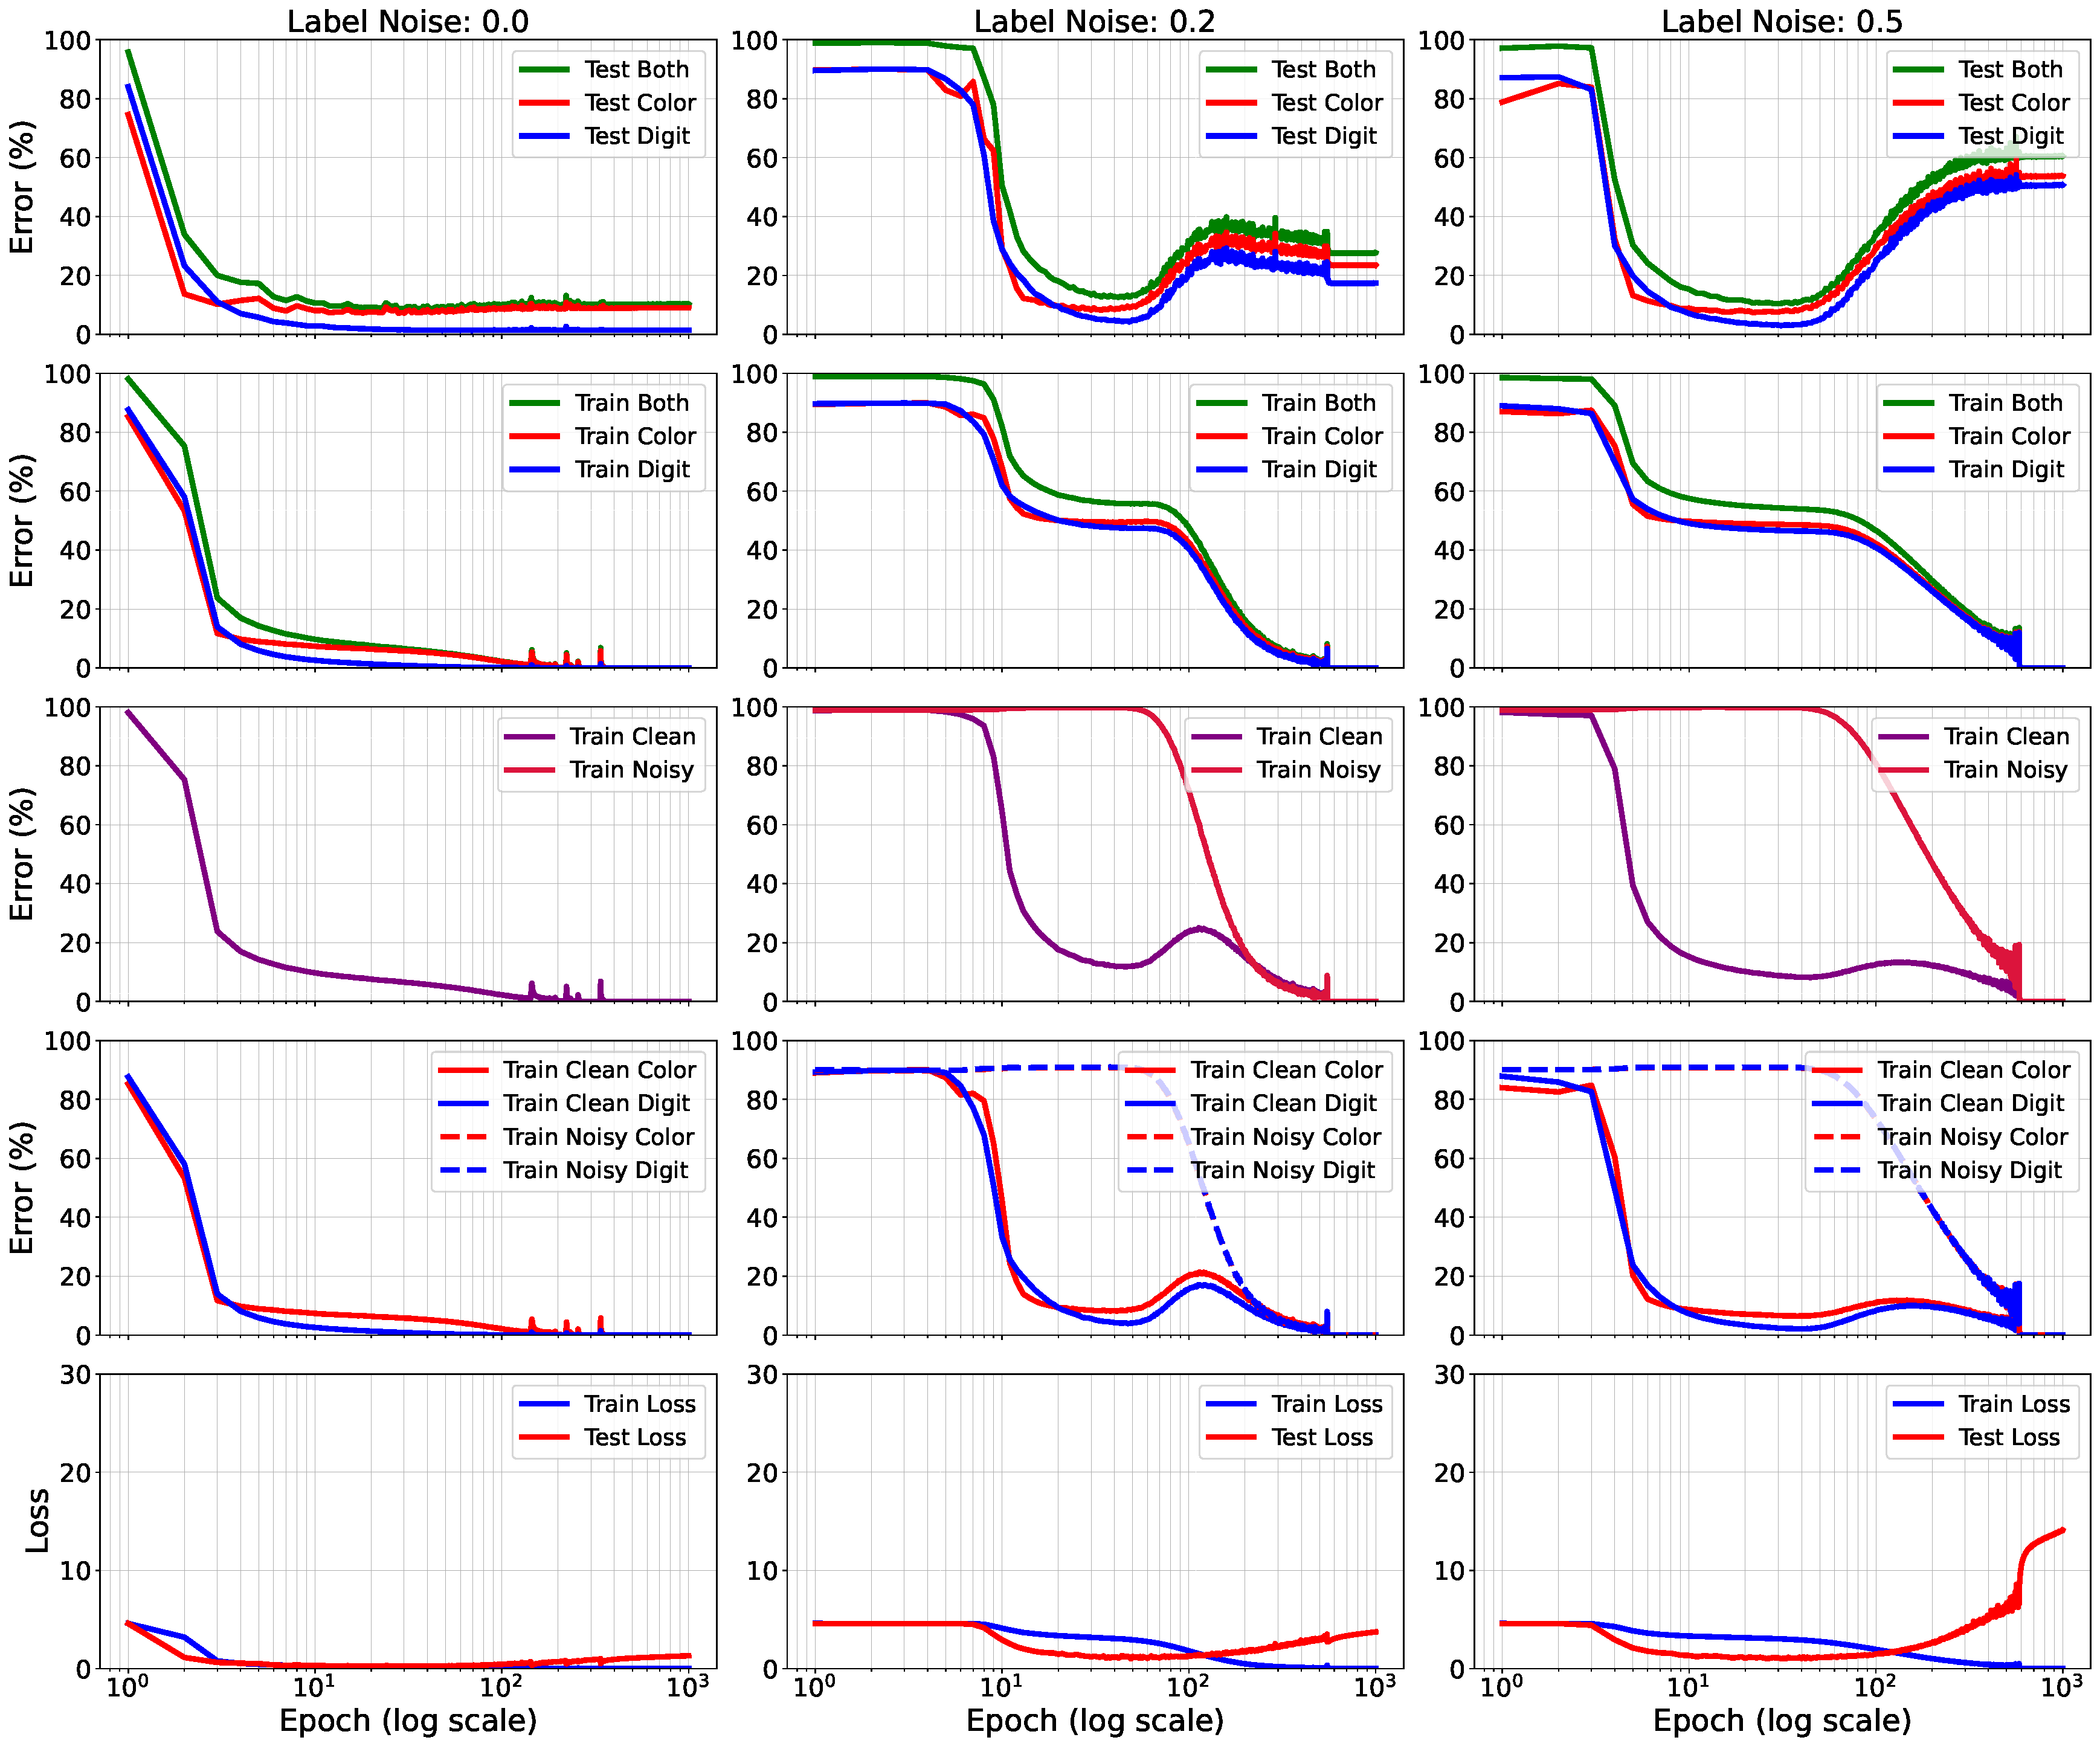
\includegraphics[width=\linewidth]{fig/erroe_metrics_by_variances/error_metrics_by_label_noise_variance_1000.pdf}
    \caption{$\sigma^2 = 10^2$のときのそれぞれのラベルノイズにおける結果}
    \label{fig:errors_by_label_noise_variance_1000}
\end{figure}

\begin{figure}[H]
    \centering
    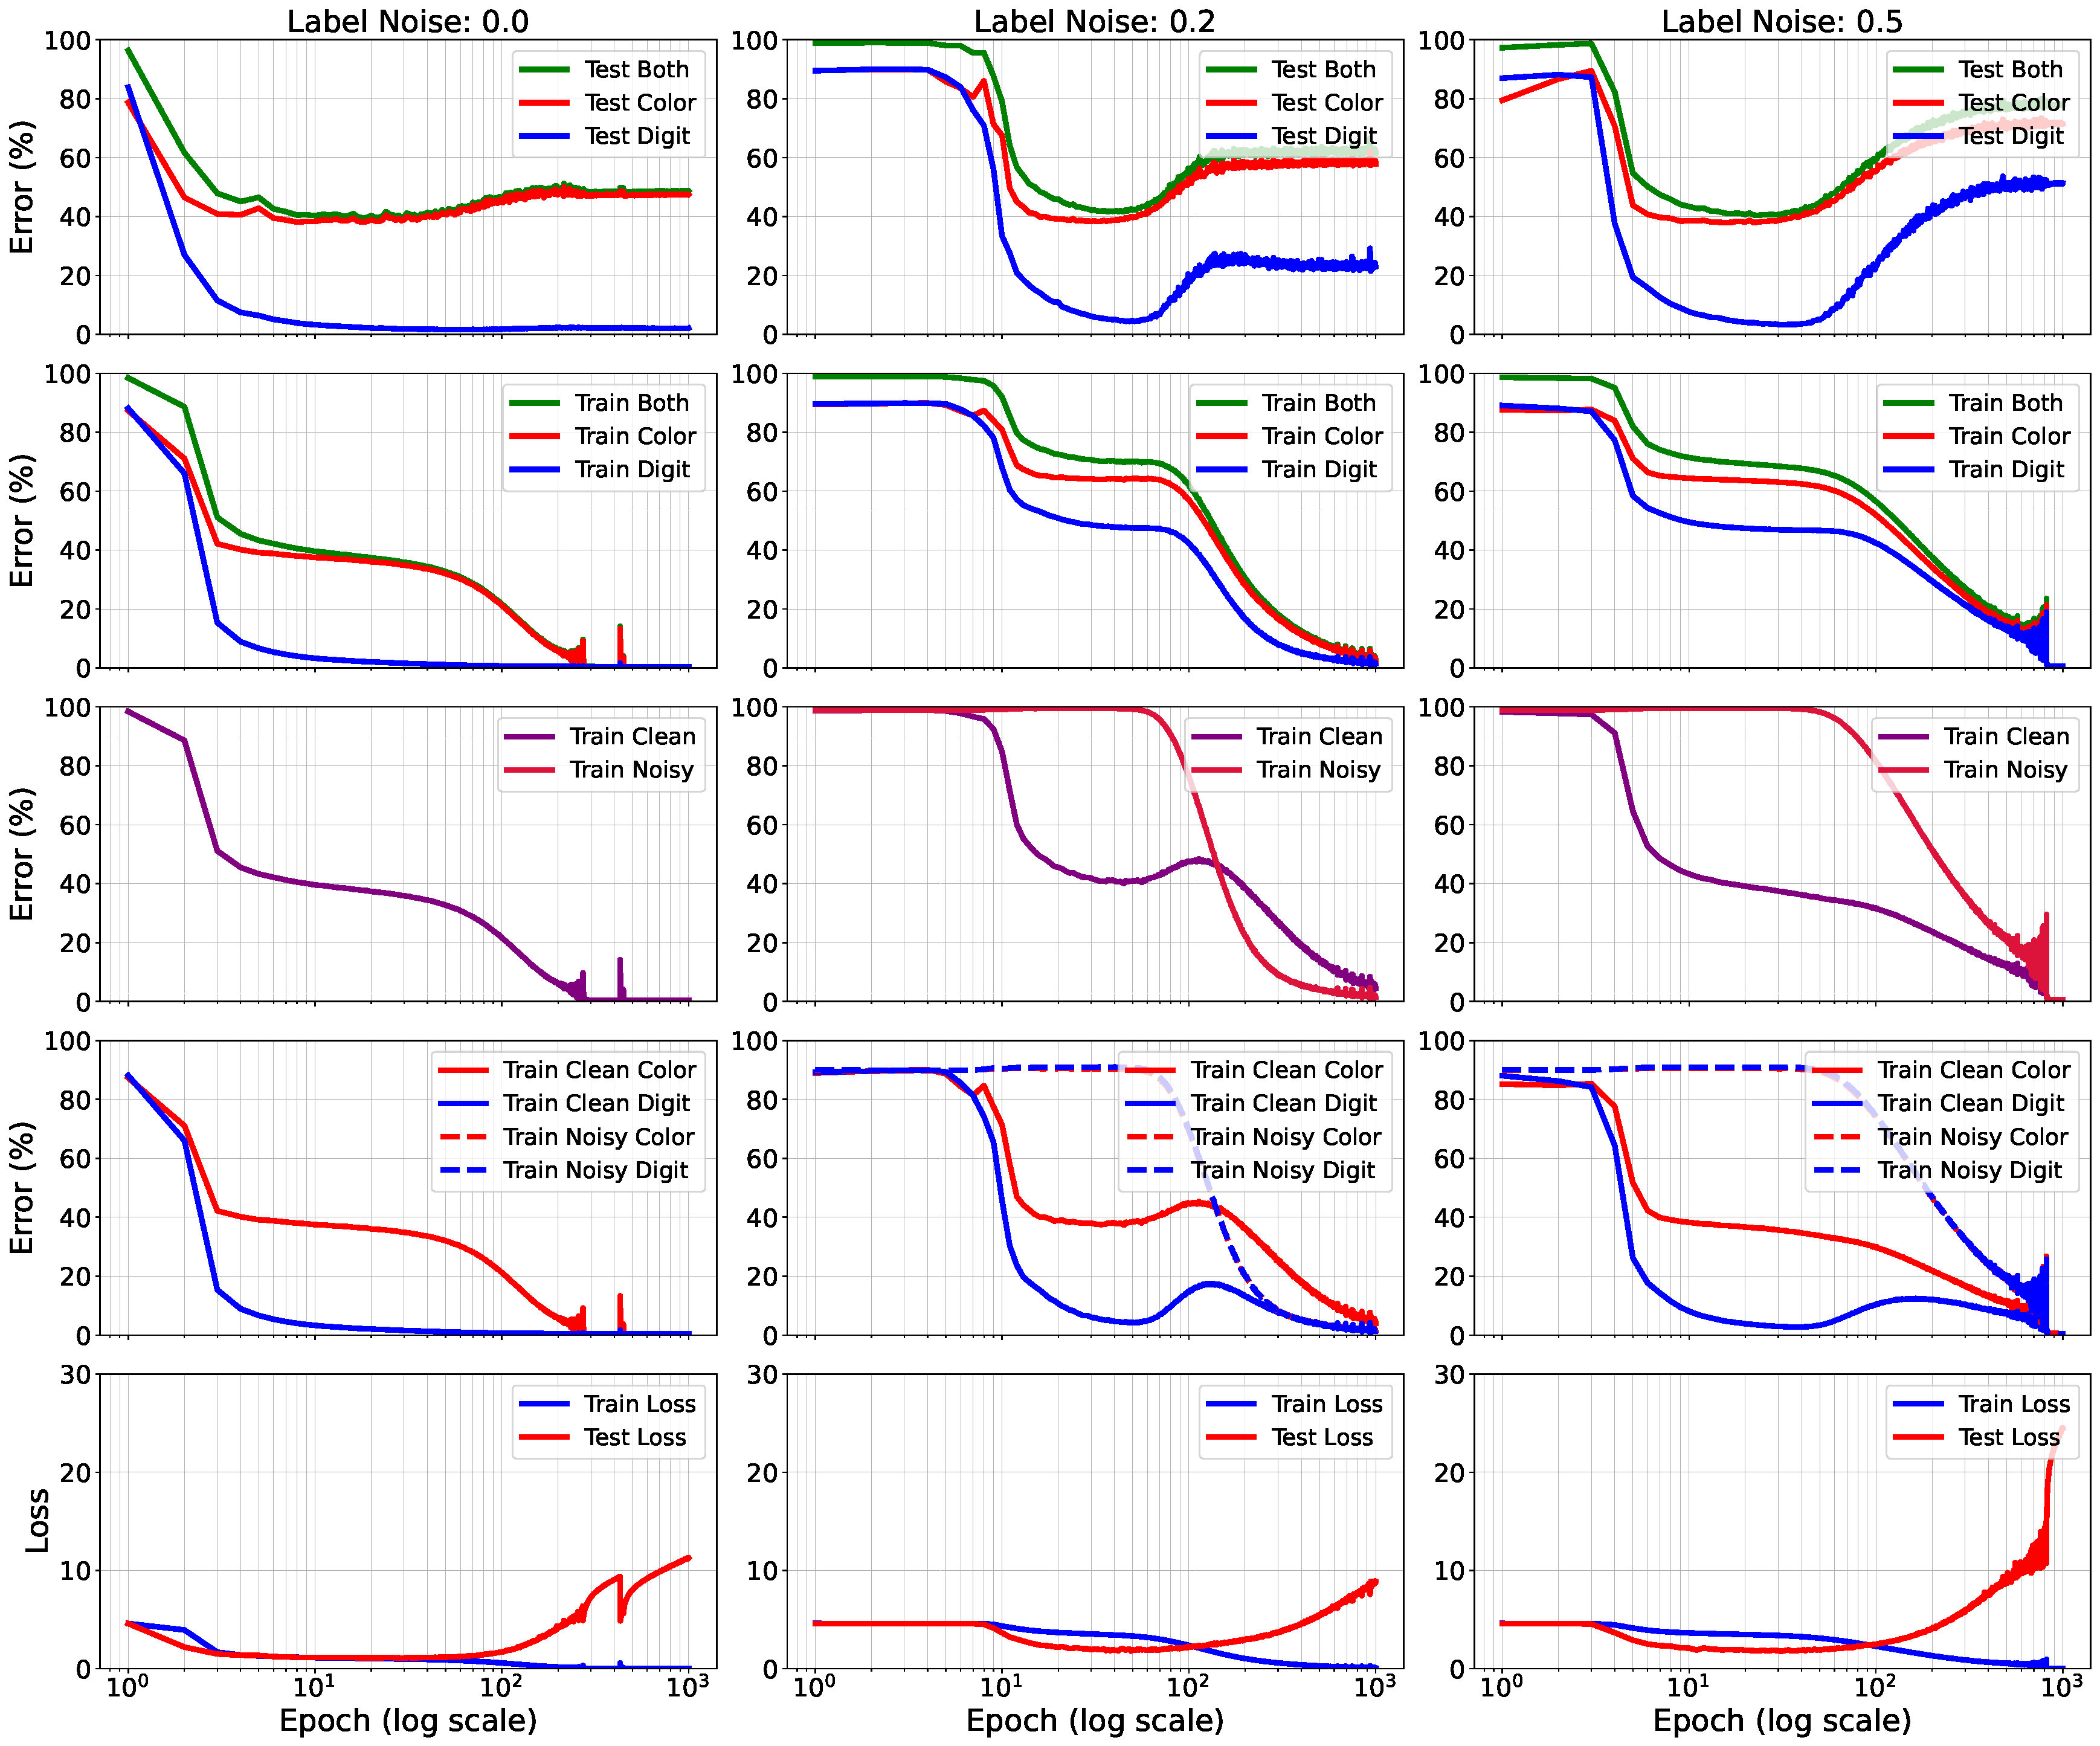
\includegraphics[width=\linewidth]{fig/erroe_metrics_by_variances/error_metrics_by_label_noise_variance_3612.pdf}
    \caption{$\sigma^2 = 10^{3.5}$のときのそれぞれのラベルノイズにおける結果}
    \label{fig:errors_by_label_noise_variance_3612}
\end{figure}

\begin{figure}[H]
    \centering
    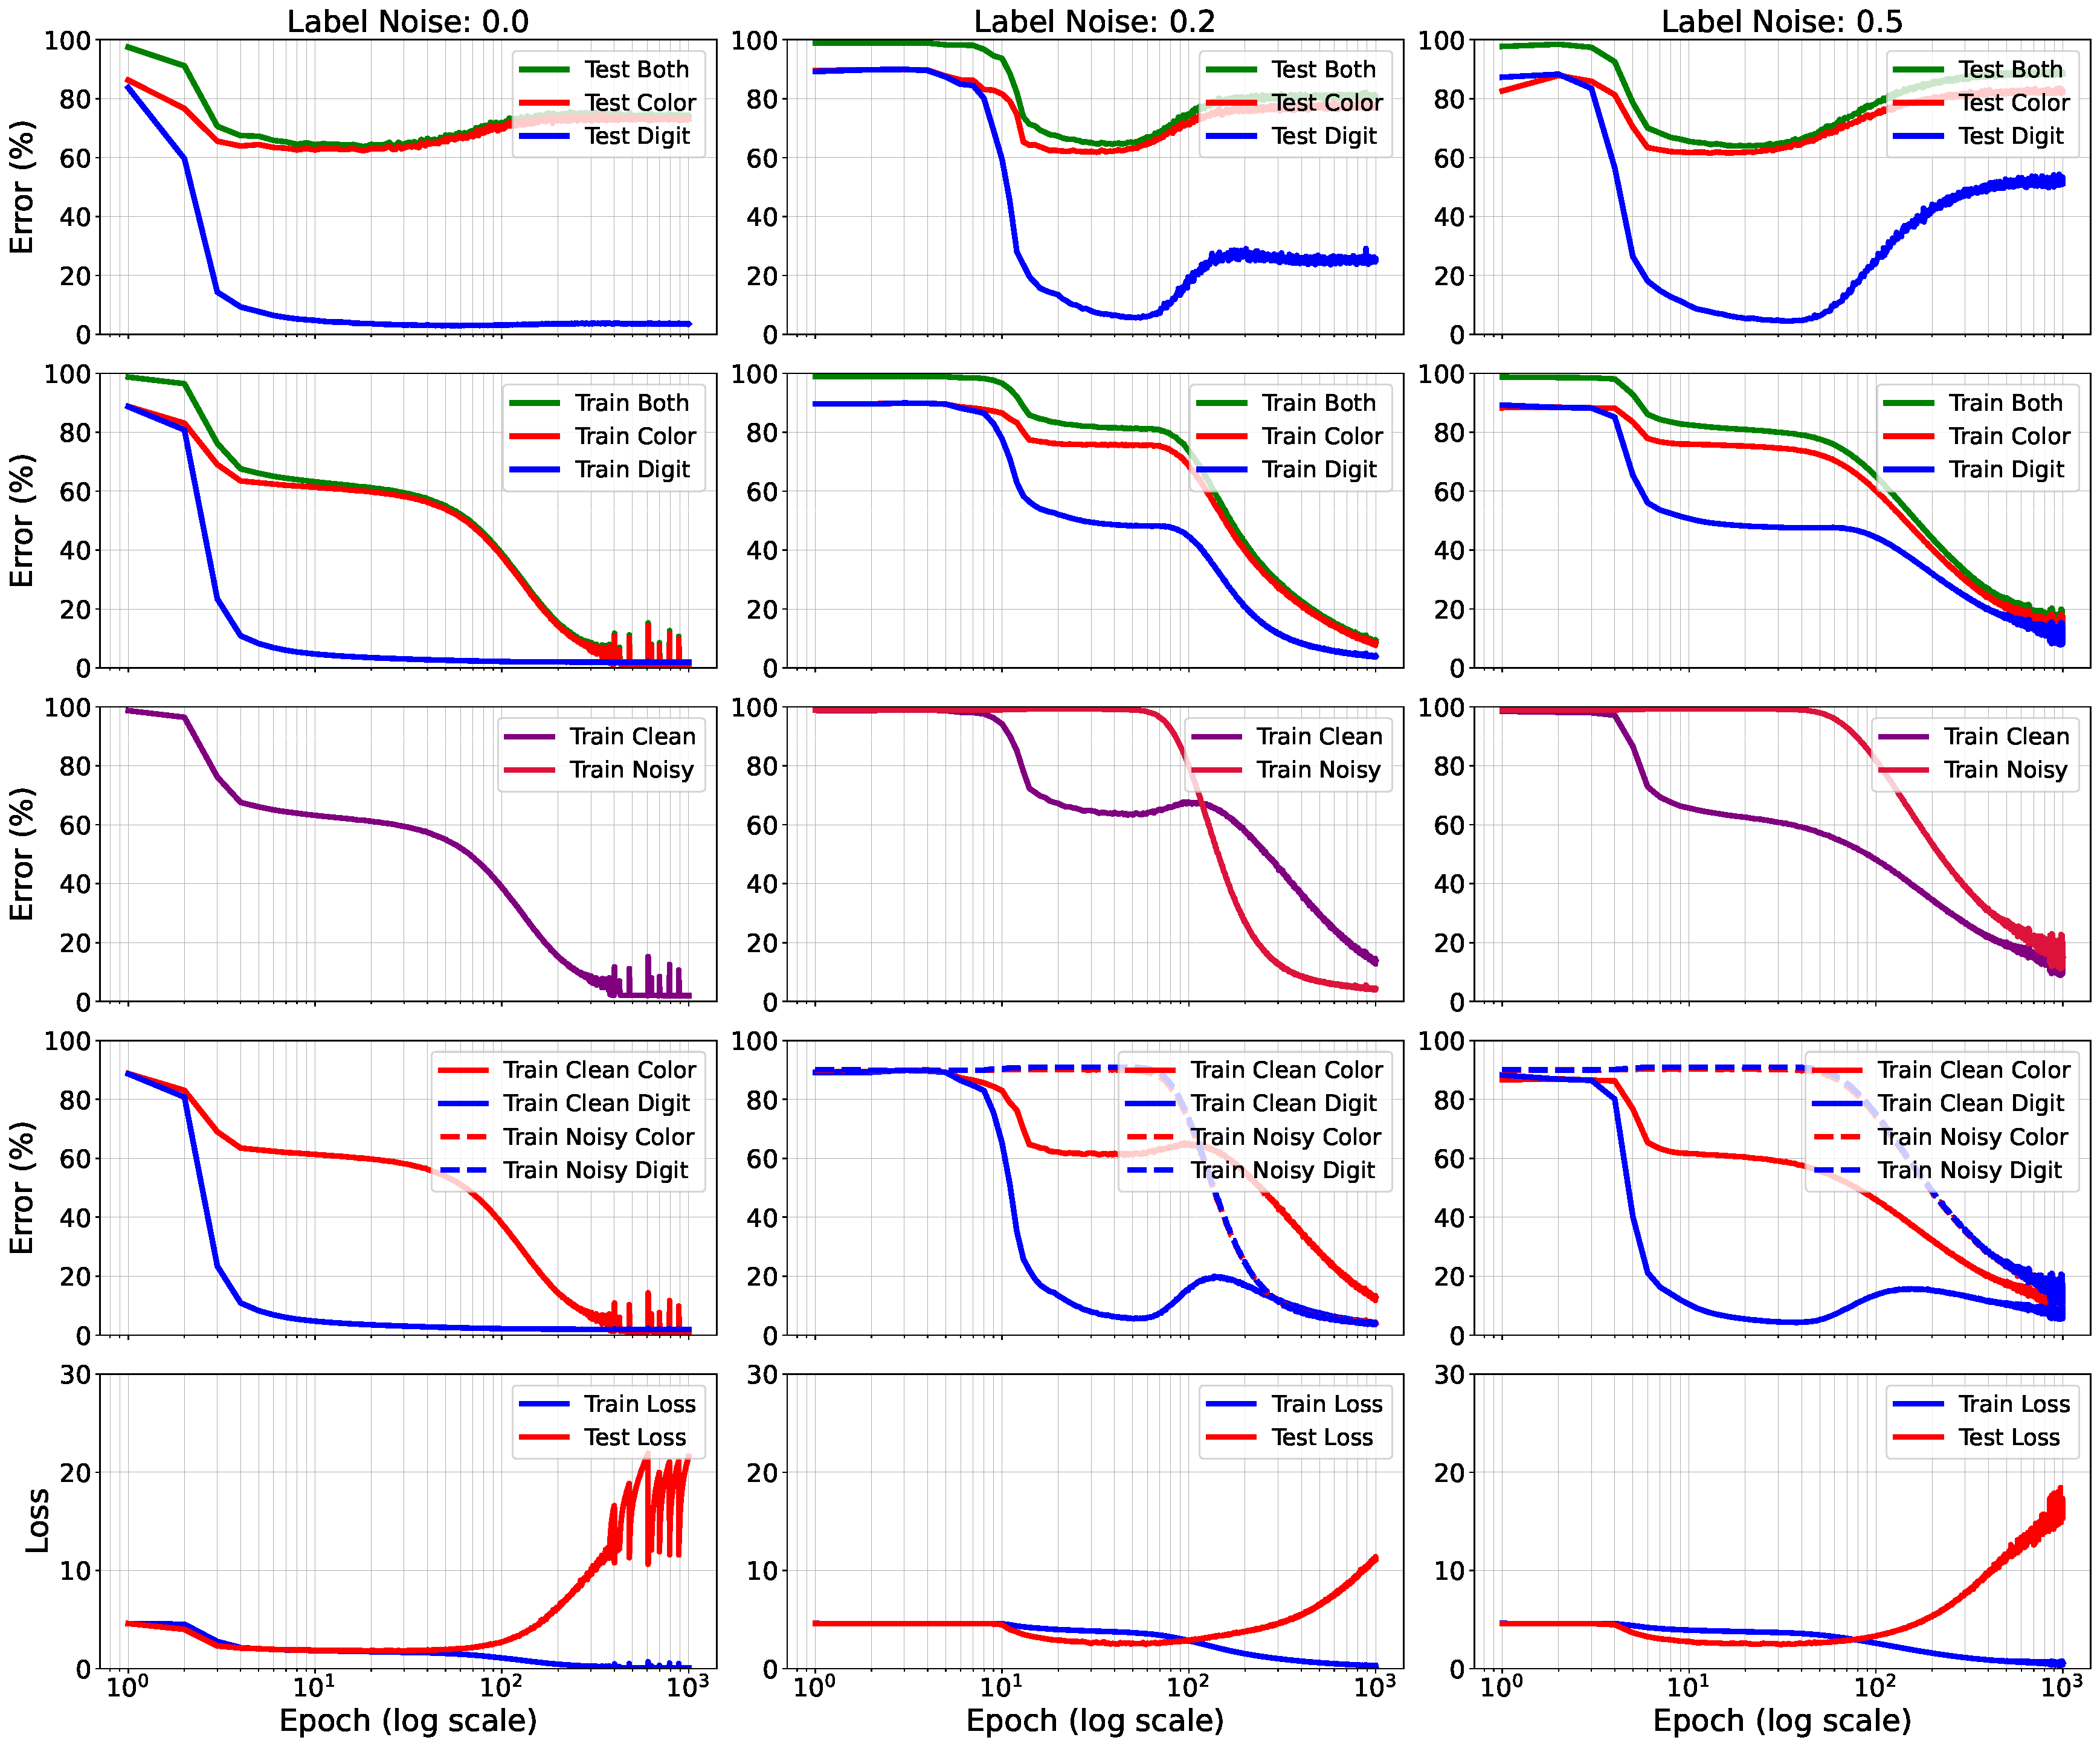
\includegraphics[width=\linewidth]{fig/erroe_metrics_by_variances/error_metrics_by_label_noise_variance_10000.pdf}
    \caption{$\sigma^2 = 10^4$のときのそれぞれのラベルノイズにおける結果}
    \label{fig:errors_by_label_noise_variance_10000}
\end{figure}

\begin{figure}
    \centering
    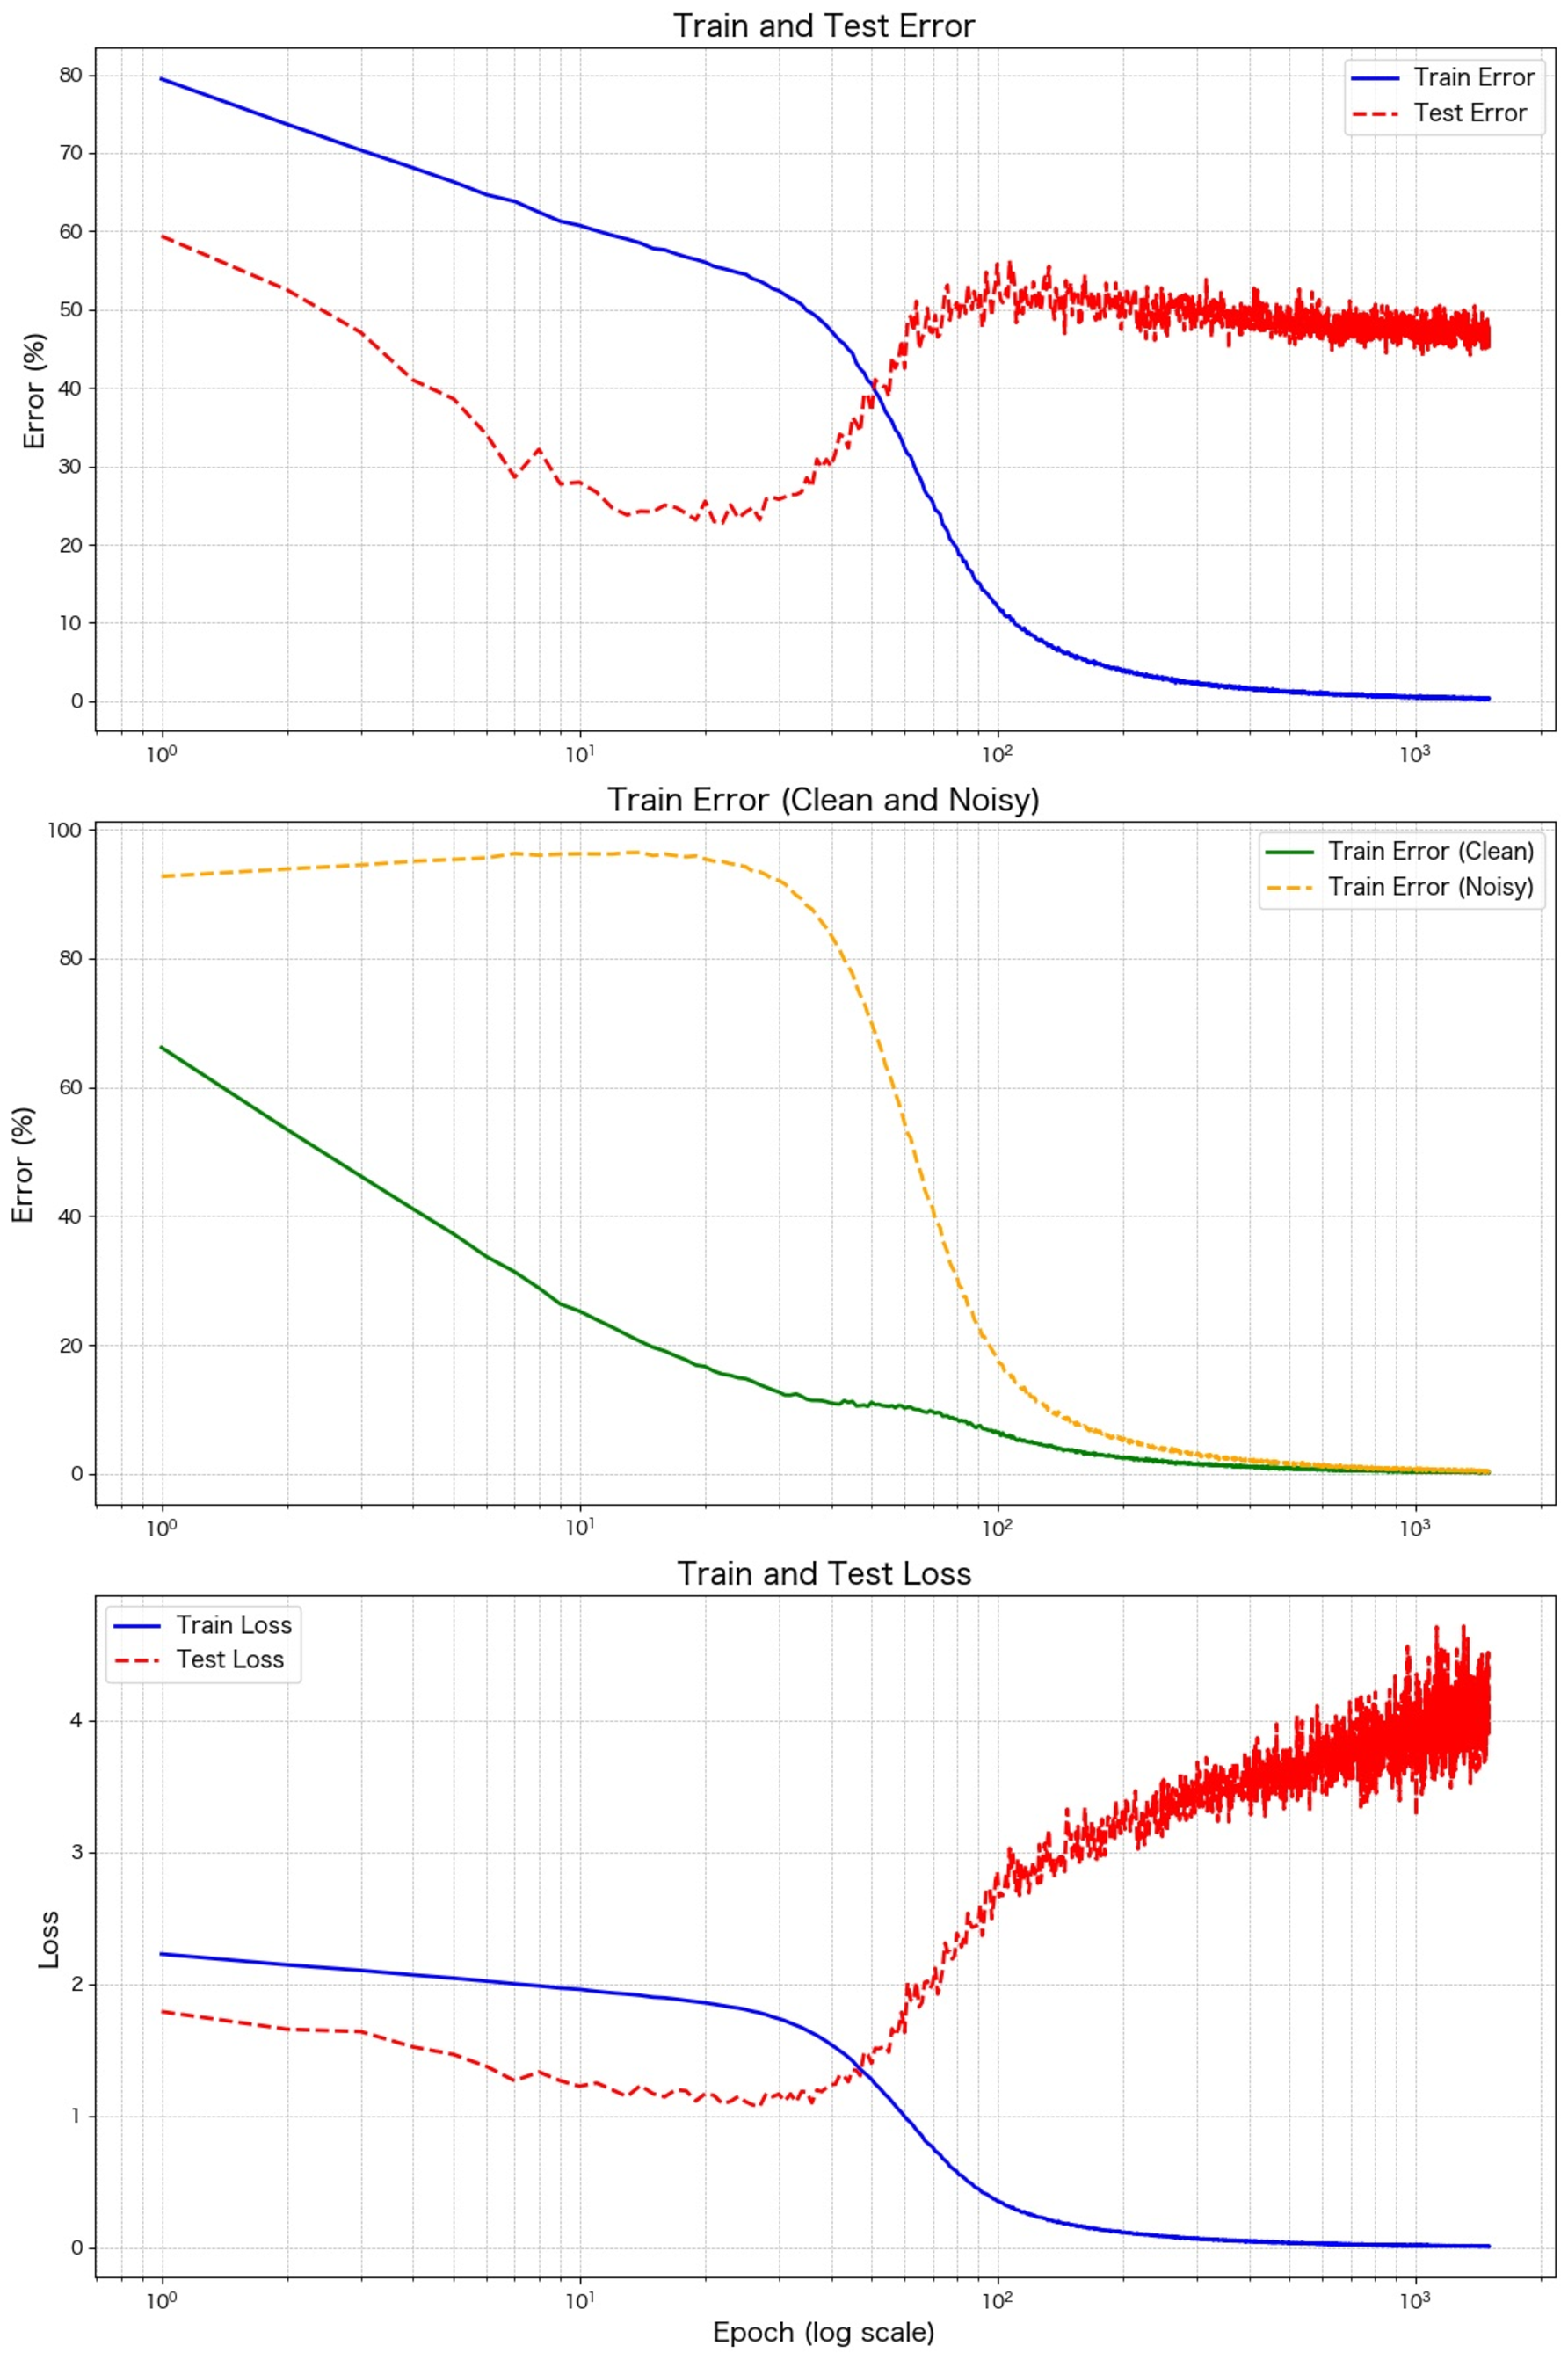
\includegraphics[width=\linewidth]{fig/nakkiran_resnet18_clean_noisy.pdf}
    \caption{Nakkiranの設定による,ラベルノイズあり・なしに分けた結果}
    \label{fig:nakkiran_resnet18_clean_noisy}
\end{figure}

\newpage

\subsection{モデルの層による変化}
8 層のCNN では,より深い層構造がもたらす効果が確認できる.図\ref{fig:5layer_results},図\ref{fig:8layer_results}
に$\gamma = 0.2,\sigma^2 = 0$の層による比較を示す.
Phase1 において,テスト誤り率はより遅いタイミングでに低下し始める.そして,5層のCNNに比べ,テスト誤り率の上昇が抑制された.
Phase3 においてはテスト誤り率の緩やかな上昇がさらに軽減される結果となった.また,8層のCNNでもラベルノイズなしデータに対して二重降下現象が観測されたが,
その程度は5 層のCNN よりも小さく,より安定した学習が行われたことが示唆される.

\begin{figure}[H]
    \centering
    \begin{minipage}[t]{0.48\linewidth}
        \centering
        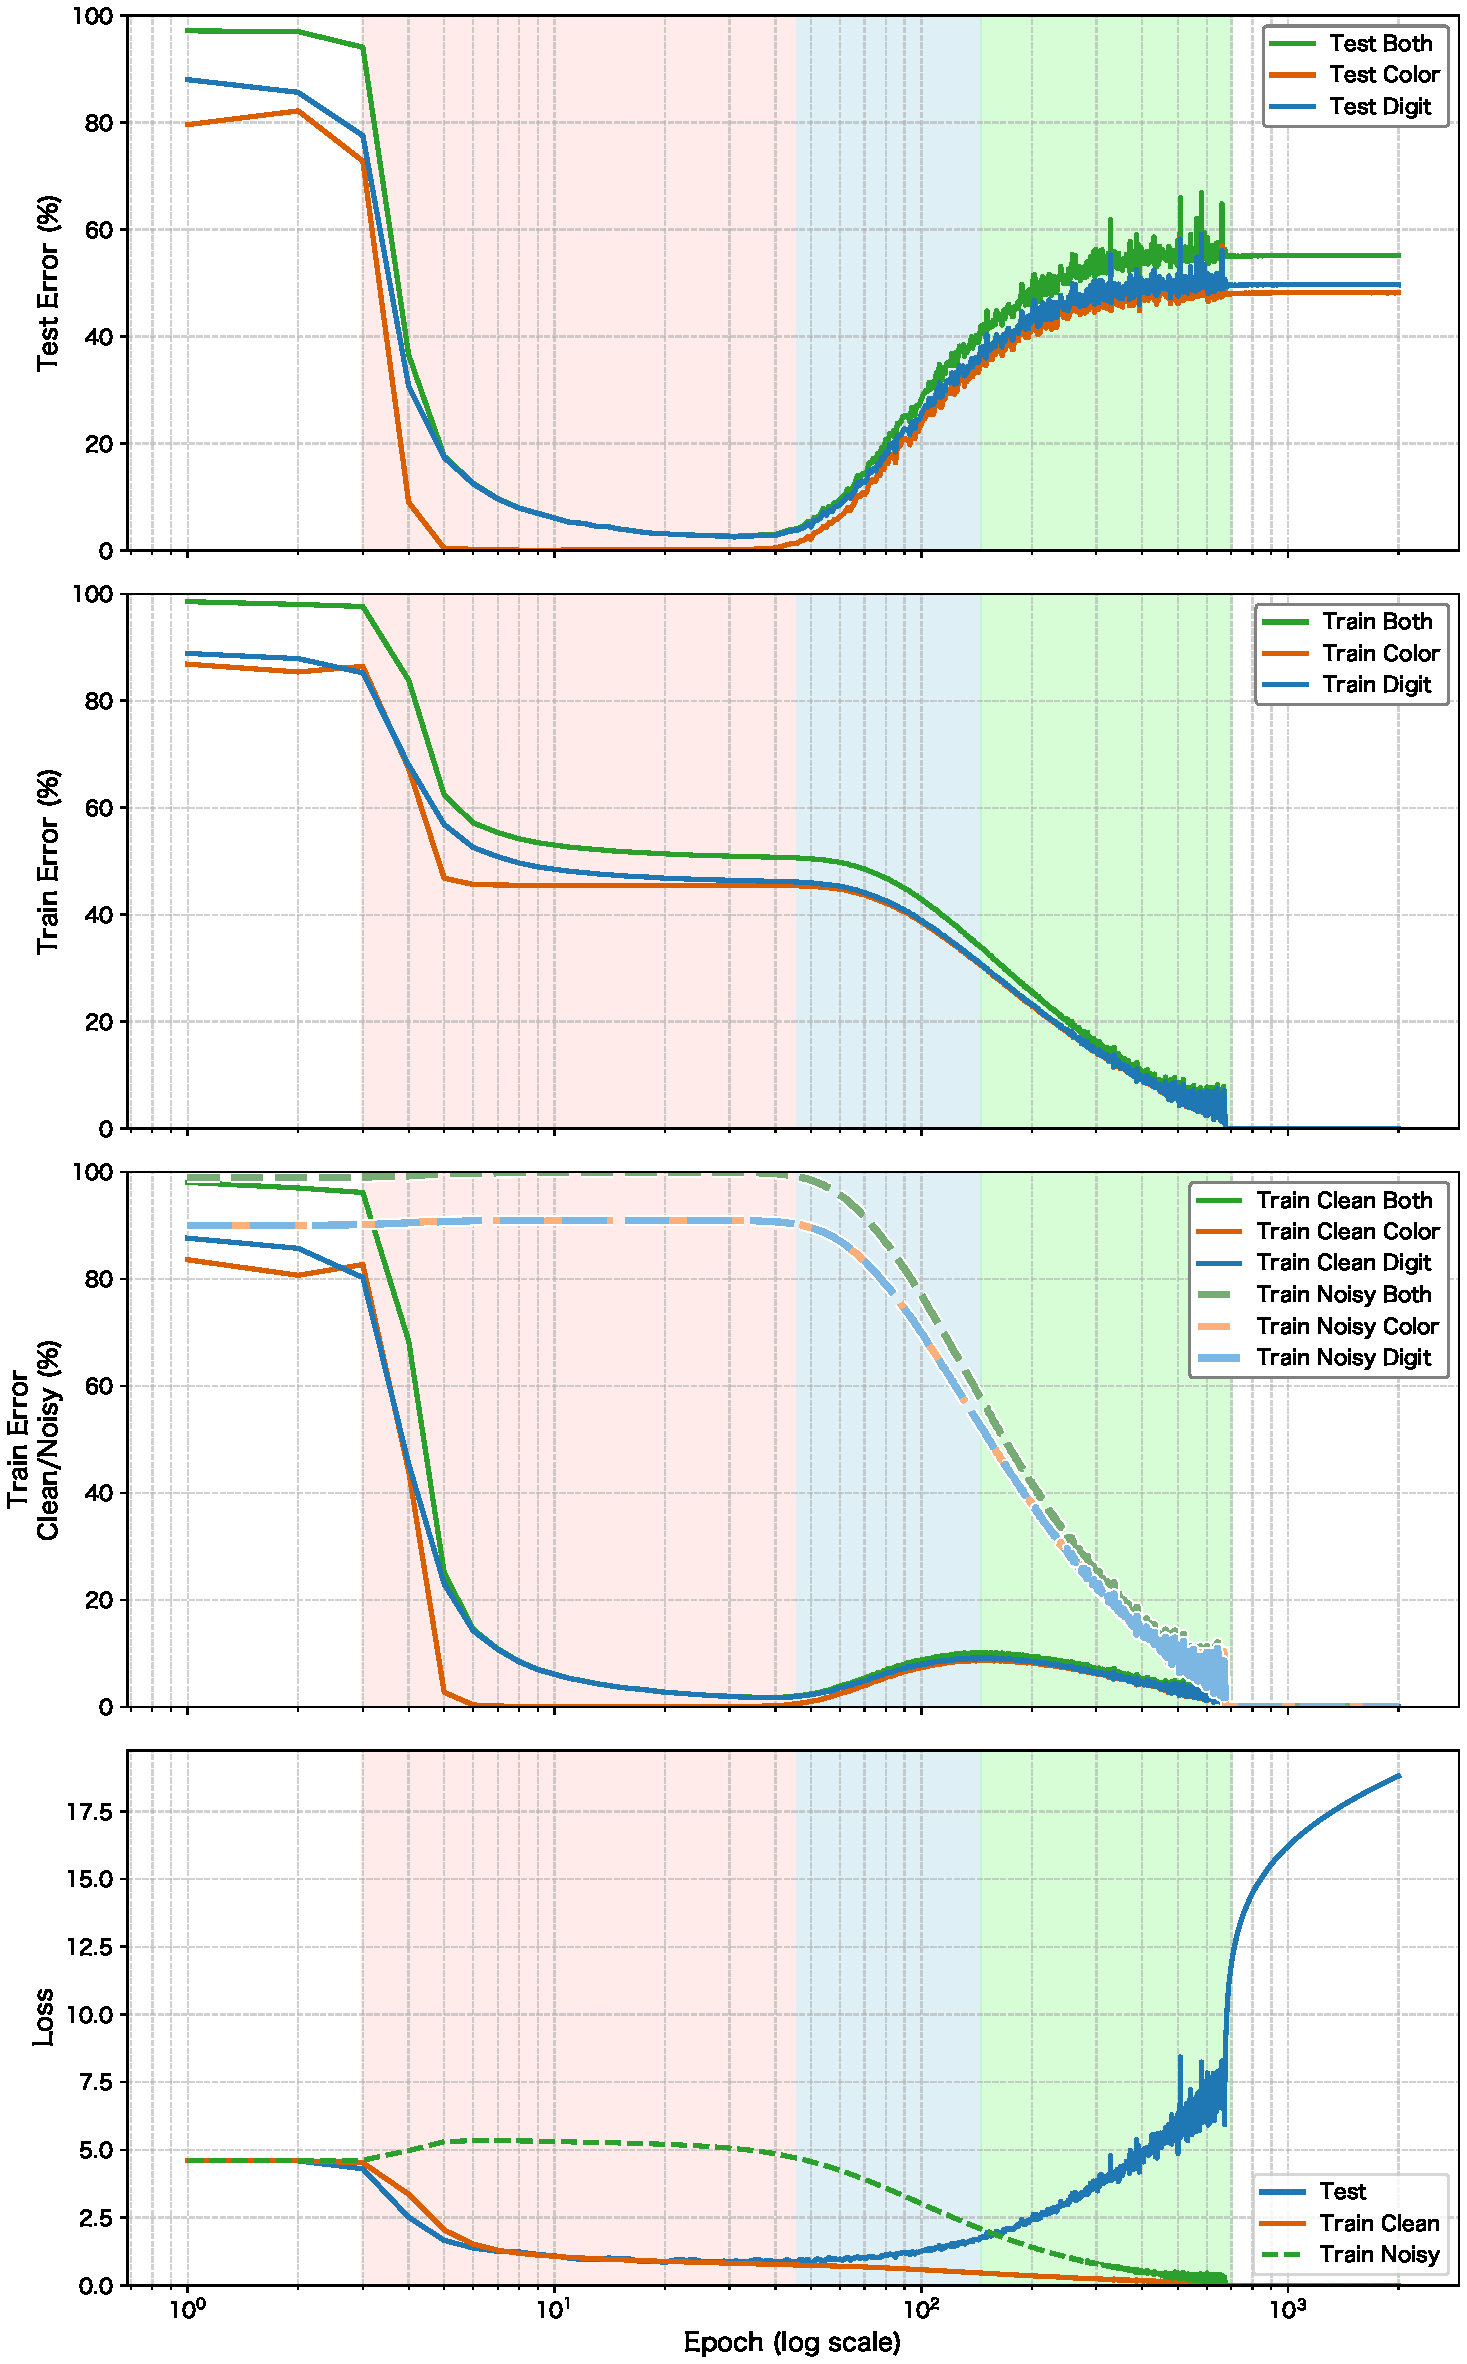
\includegraphics[width=\linewidth]{fig/layer_comparison/cnn5_error_comp_layer.pdf}
        \caption{5層のCNNモデルの100クラス分類タスクにおけるそれぞれの誤り率($\gamma = 0.5$)}
        \label{fig:5layer_results}
    \end{minipage}
    \hfill
    \begin{minipage}[t]{0.48\linewidth}
        \centering
        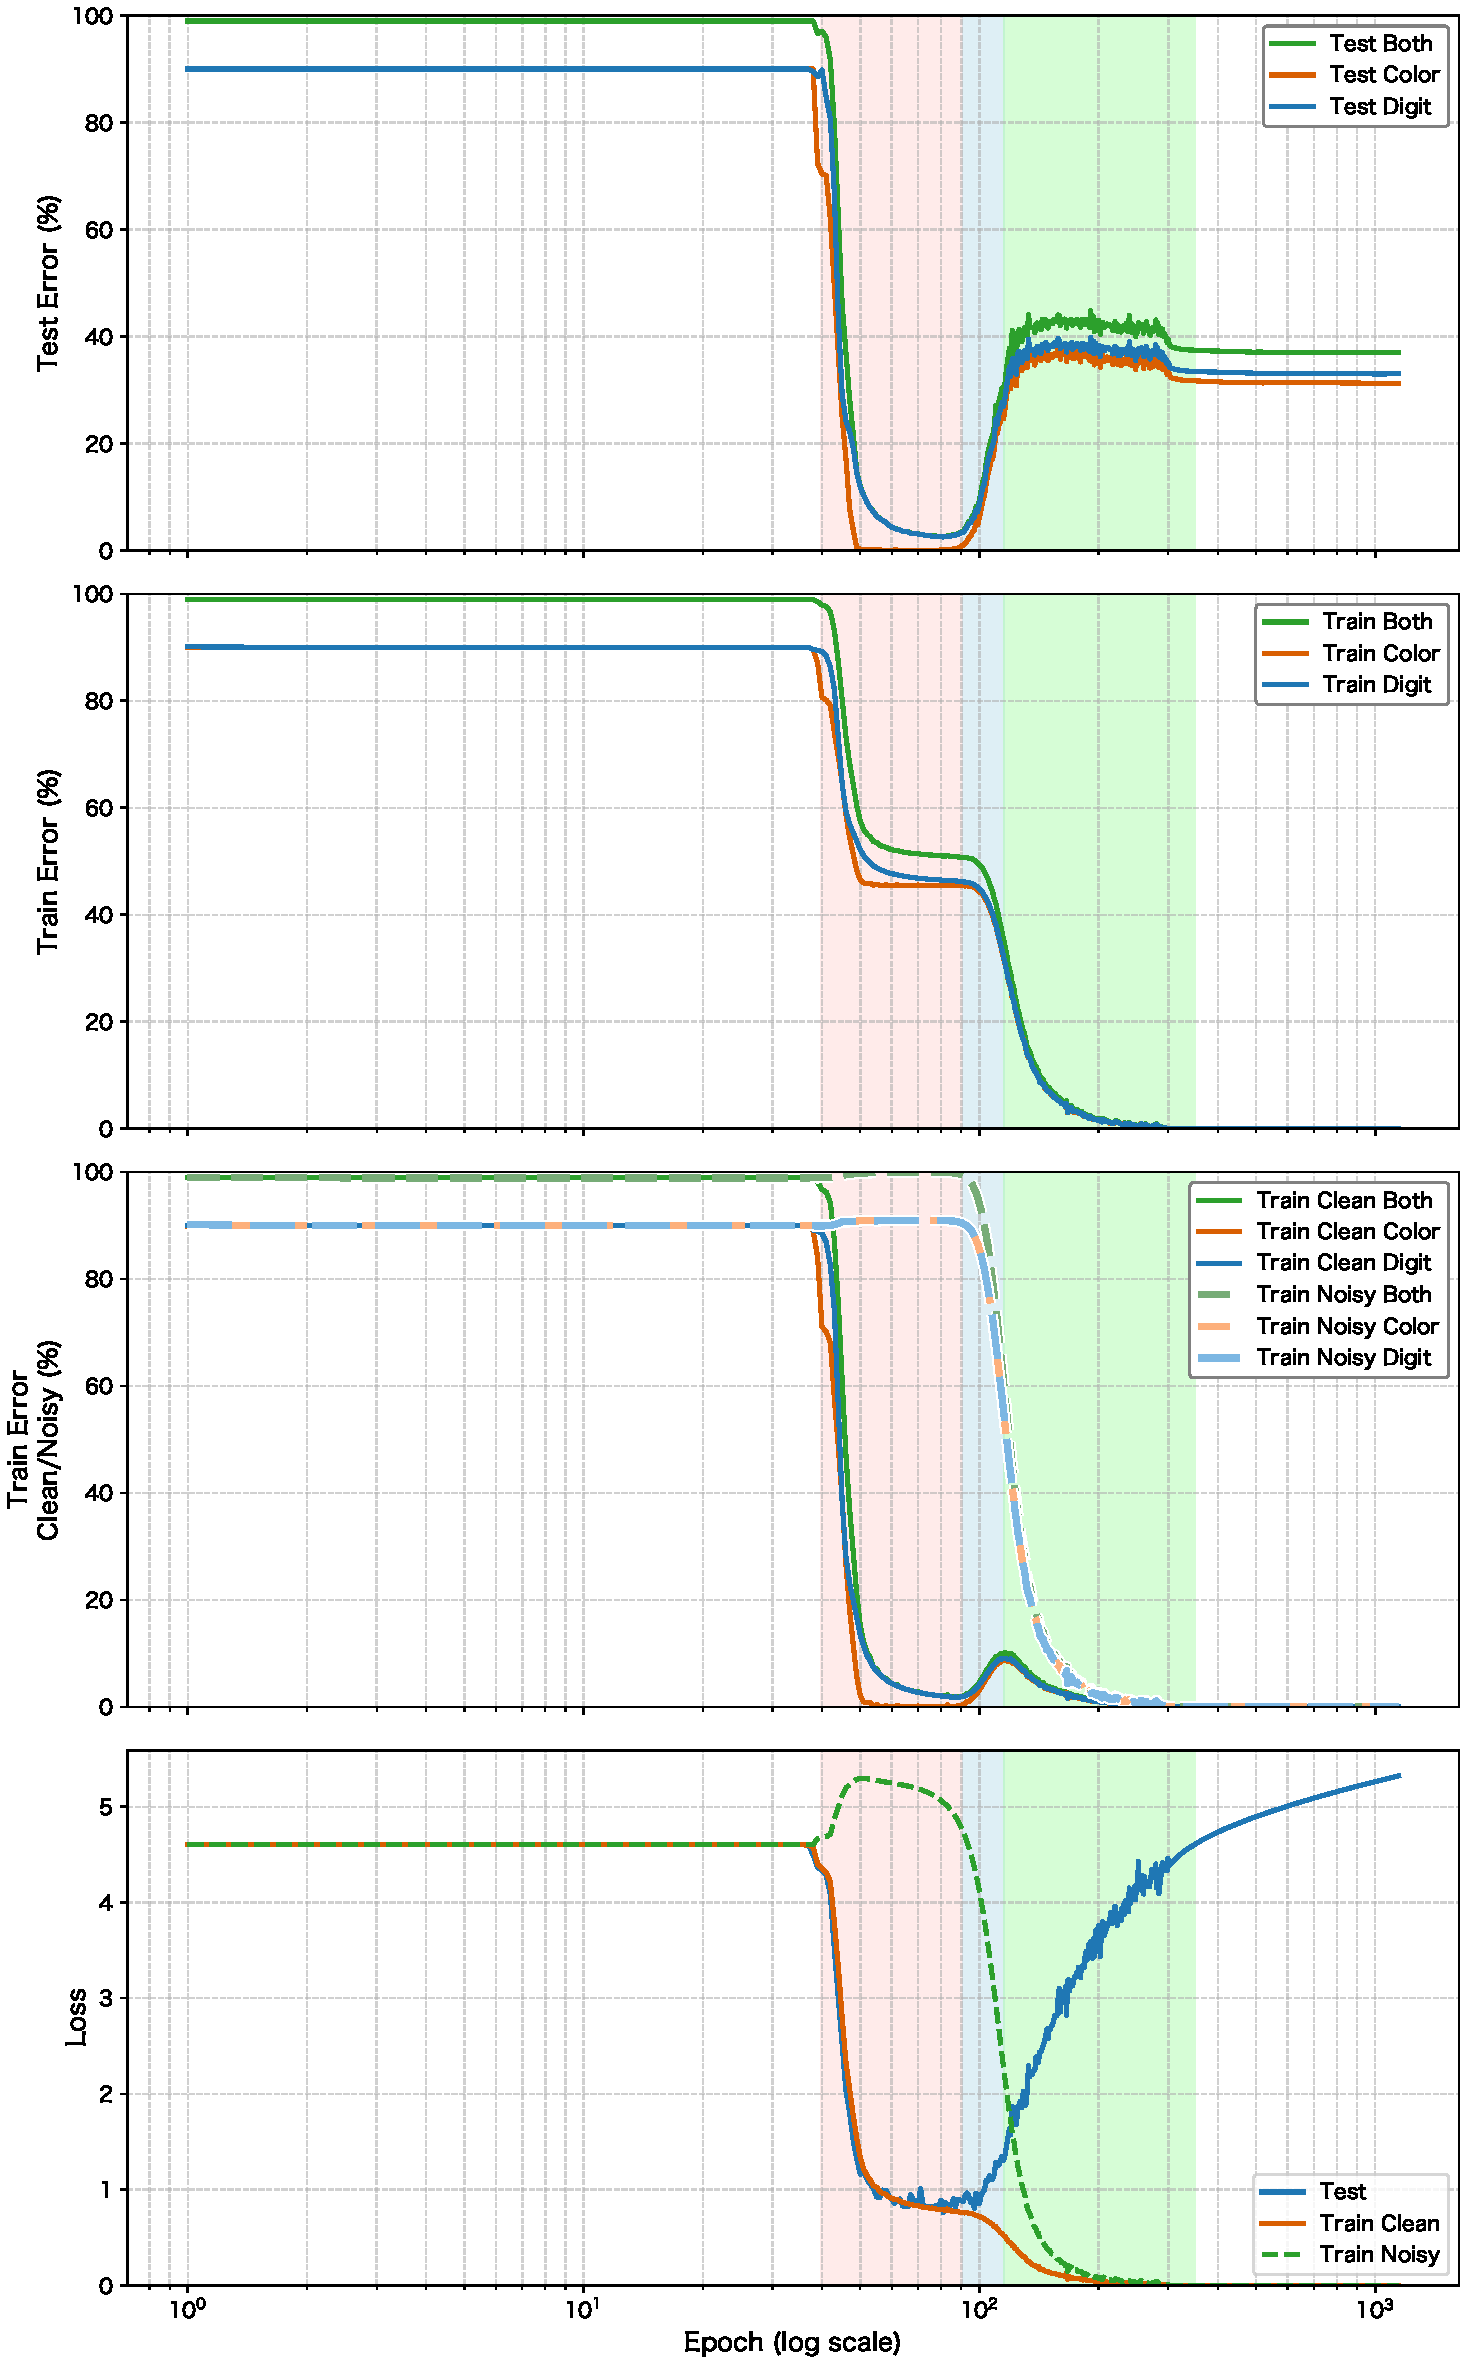
\includegraphics[width=\linewidth]{fig/layer_comparison/cnn8_error_comp_layer.pdf}
        \caption{8層のCNNモデルの100クラス分類タスクにおけるそれぞれの誤り率($\gamma = 0.5$)}
        \label{fig:8layer_results}
    \end{minipage}
\end{figure}

また,図\ref{fig:cnn_layers_comparison}に2,3,5,8,16層のCNNモデルのそれぞれの誤り率を示す.
CNNモデルの層数による性能評価の実験結果について,以下の重要な知見が得られた.

2層モデルは,学習の初期段階で比較的速い誤差の減少を示したものの,最終的な性能は他のモデルと比較して限定的であった.
特に,訓練エラー率とテストエラー率の両方において約\SI{40}{\percent}程度で停滞し,モデルの表現力の限界を示唆する結果となった.
3層モデルは2層モデルと同様に,早期の学習段階でエラー率の減少を示したが,最終的なエラー率は約\SI{30}{\percent}付近で収束した.
このことは,層数の微増による性能向上の効果が限定的であることを示している.
5層と8層のモデルは,比較的早い段階(10エポック付近)でエラー率が\SI{20}{\percent}以下まで低下し,安定した学習を示した.
特に8層モデルは,色と数字の両タスクにおいて最も安定した学習を示し,最終的な誤差も比較的低い水準で収束した.
16層モデルは特徴的な学習パターンを示した.学習の初期段階($10^2$エポック以前)では誤差の改善がほとんど見られず,その後急激な性能向上を示すという段階的な学習曲線を描いた.
また,学習後期($10^3$エポック以降)では損失値の大きな振動が観察され,過学習の傾向が最も顕著であった.
さらに,ノイズを含むデータに対する性能低下が他のモデルと比較して著しく,モデルの深さと頑健性のトレードオフが明確に表れる結果となった.
この実験結果から,単純にモデルの層を深くすることが必ずしも性能向上につながるわけではなく,タスクの複雑さに応じて適切な層数を選択することの重要性が示唆された.

\begin{figure}[H]
    \centering
    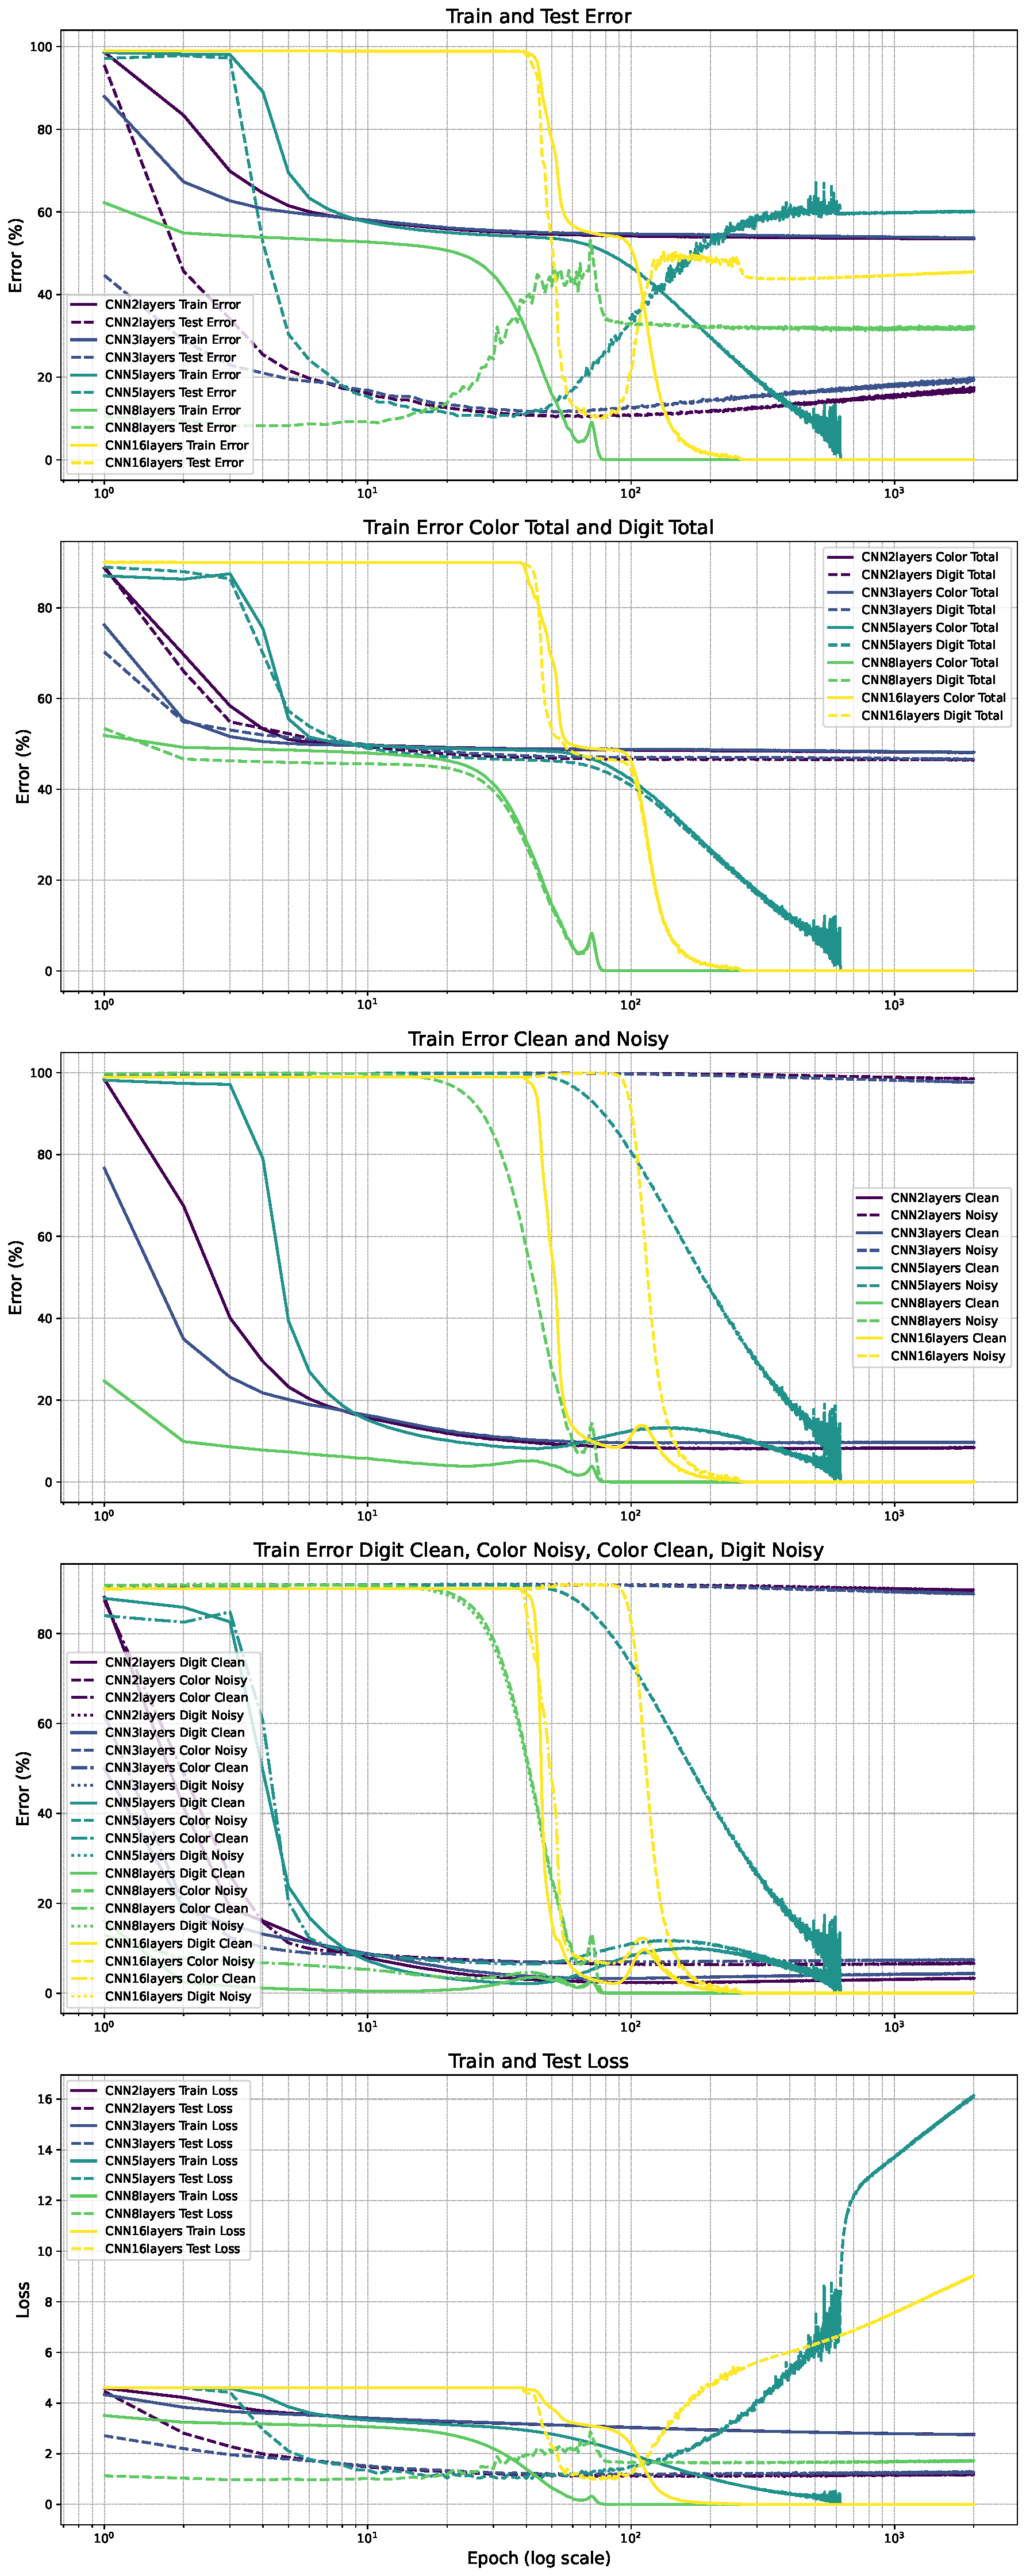
\includegraphics[width=0.4\linewidth]{fig/layer_comparison/cnn_layers_comparison.pdf}
    \caption{$\gamma = 0.5, \sigma^2 = 10^3$,のときのCNNの層の深さによる比較}
    \label{fig:cnn_layers_comparison}
\end{figure}

\newpage

\subsection{モデル幅による変化}

CNNのチャネル幅(Width)がモデルの性能に与える影響について,以下の実験結果が得られた.
結果を図\ref{fig:modelwidth_ln02}に示す.

Width 1のモデルは,訓練エラー率とテストエラー率の両方において,学習の収束が最も遅く,
最終的なテストエラー率も約\SI{20}{\percent}と高い値を示した.
特筆すべき点として,$10^2$エポック以降で訓練エラー率が\SI{0}{\percent}近くまで減少する一方で,
テストエラー率は高止まりしており,早期の段階で過学習が発生していることが確認された.
これは,チャネル幅が狭すぎることによるモデルの表現力の不足を示唆している.興味深いことに,カラー情報のノイズに対して特に脆弱性を示したが,
これはチャネル幅の狭さにより色空間の複雑な特徴を十分に捉えられていないことが原因として考えられる.

Width 2およびWidth 4のモデルは,10エポック付近から徐々に性能が向上し始め,
最終的なテストエラー率は\SI{10}{\percent}程度まで改善した.Width 1と比較すると過学習の発生が遅く,
特にWidth 4のモデルは,カラー情報と数字情報の両タスクにおいて安定した学習を示した.しかしながら,
$10^2$エポック以降では,これらのモデルにおいても訓練エラー率とテストエラー率の乖離が徐々に大きくなり,
緩やかな過学習の傾向が観察された.特に注目すべき点として,Width 4モデルではノイズの有無による性能差がWidth 2モデルより小さく,
これはチャネル幅の拡大がモデルの特徴抽出能力を向上させることを示唆している.

Width 8のモデルは,最も早い段階(1エポック付近)から急速な性能向上を示し,
最終的なテストエラー率は\SI{5}{\percent}未満という最も優れた性能を達成した.
また,訓練ロスとテストロスの推移も安定しており,他のモデルと比較して過学習の傾向が最も抑制されていることが確認された.
これは,適切なチャネル幅が,モデルの表現力と汎化性能のバランスを最適化できることを示唆している.
さらに,Width 8モデルは学習の初期段階における損失の減少が最も急峻であり,
これは十分な幅を持つチャネルが効率的な特徴学習を可能にすることを示している.
ノイズの影響に関する分析では,チャネル幅が広いモデルほどノイズに対する頑健性が高いことが示された.
特にWidth 8のモデルは,ノイズを含むデータに対しても安定した性能を維持し,
クリーンなデータとノイズを含むデータの間のエラー率の差が最も小さかった.
特筆すべき点として,カラー情報のノイズに対する頑健性がWidth 8モデルで顕著に高く,
これは広いチャネル幅により,ノイズの影響を受けにくい堅牢な特徴表現を学習できていることを示唆している.
一方,Width 1のモデルでは,ノイズの有無によって大きな性能差が生じ,特にカラー情報のノイズに対して脆弱性を示した.
また,ノイズを含むデータセットでは,全てのモデルにおいて過学習の発生が早まる傾向が観察された.
数字認識タスクとカラー認識タスクの比較において,興味深い傾向が観察された.全てのモデルにおいて,
カラー認識タスクの方が数字認識タスクより高いエラー率を示す傾向があり,これは色空間の特徴抽出がより複雑な課題であることを示唆している.
特に,チャネル幅が狭いモデルほどこの傾向が顕著であり,カラー情報の効果的な処理には十分なチャネル幅が必要であることが明らかとなった.
これらの結果から,チャネル幅の拡大は,学習の収束速度,最終的な性能,過学習の抑制,およびノイズに対する頑健性の全ての面で有意な改善をもたらすことが示された.
特に,本実験で検証したパラメータの範囲では,Width 8が最適なチャネル幅であることが明らかとなった.さらに,タスクの複雑さとチャネル幅の関係性において,より複雑な特徴抽出を必要とするタスクほど,十分なチャネル幅が重要であることが示唆された.

\begin{figure}[H]
    \centering
    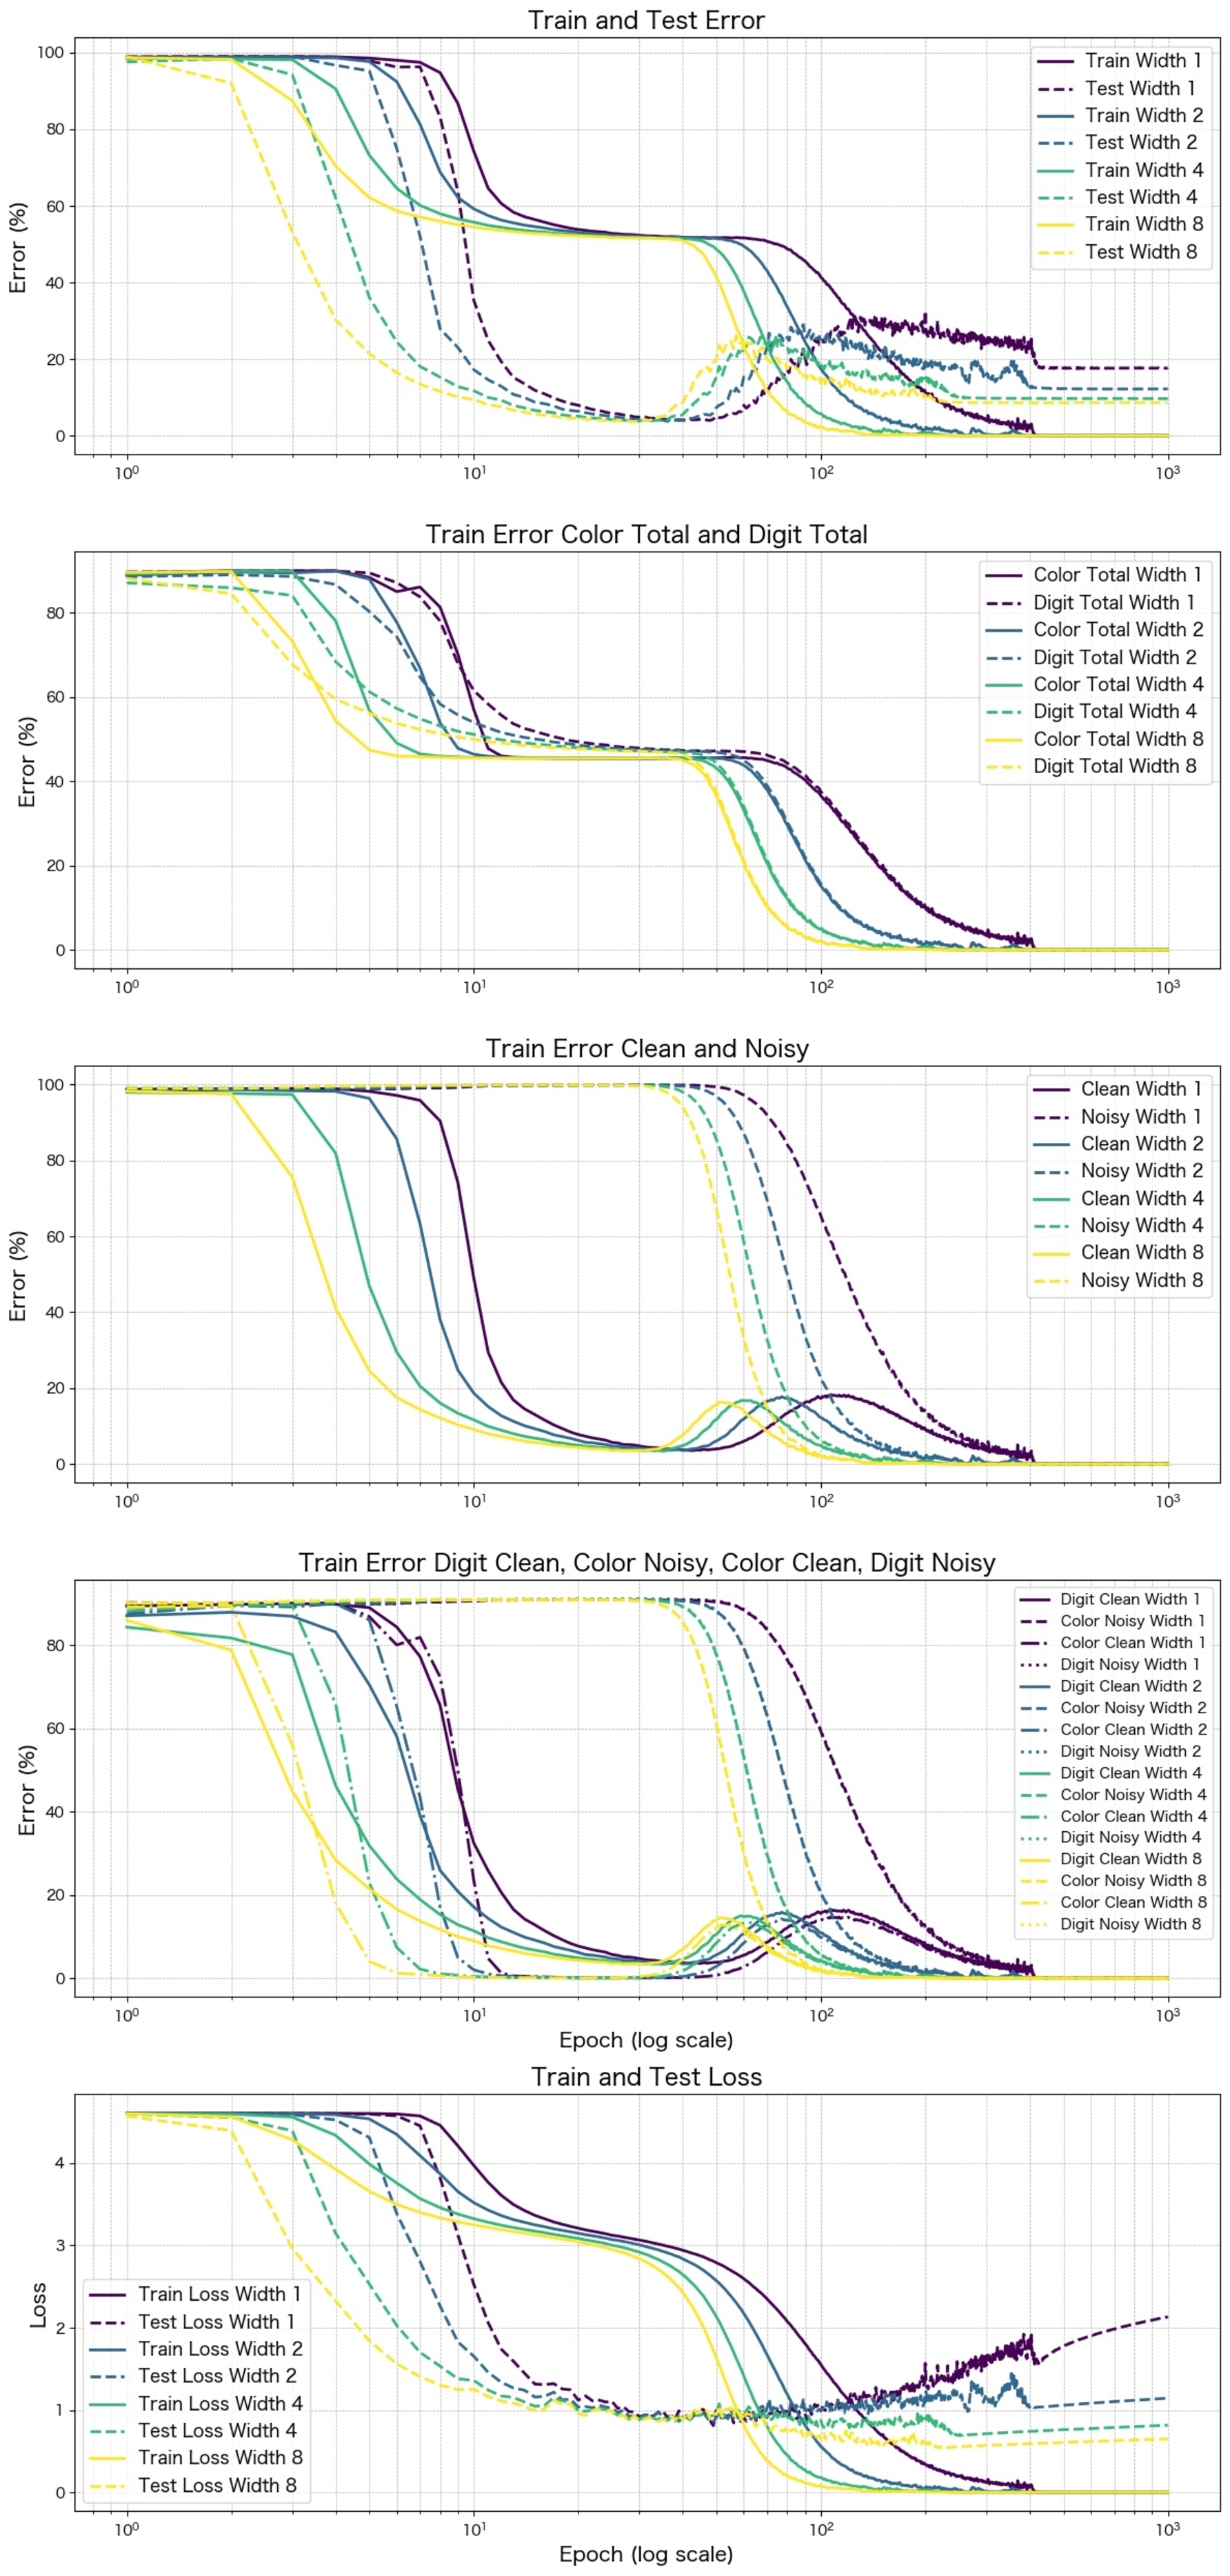
\includegraphics[width=0.5\linewidth]{fig/modelwidth_ln0.2.pdf}
    \caption{$\gamma = 0.2, \sigma^2 = 0$,のときのmodel width別の結果}
    \label{fig:modelwidth_ln02}
\end{figure}

\newpage

\subsection{チャネル幅とエポック数によるテストエラー率の分析}
また,図\ref{fig:modelwidth_heatmap}にエポックとチャネル幅の関係を表すヒートマップ示す.
テストエラー率のヒートマップ分析から,モデルのチャネル幅とエポック数の関係性について,以下の重要な知見が得られた.
チャネル幅8のモデルは,最も効率的な学習挙動を示した.具体的には,エポック10付近から急速にテストエラー率が低下し,
その後も安定して低いエラー率(約\SI{20}{\percent})を維持している.
これは,十分な表現力を持つチャネル幅の設定により,効率的な特徴抽出が可能となったことを示している.
一方,チャネル幅1および2のモデルでは,初期の学習段階(エポック1-10)において高いテストエラー率(約\SI{80}{\percent})が継続し,その後の低下も緩やかである.
特にチャネル幅1の場合,エポック100以降でテストエラー率が再び上昇する傾向が観察された.
この結果は,チャネル幅が狭すぎる場合,モデルの表現力が制限され,複雑な特徴を適切に抽出できないことを示唆している.
チャネル幅4のモデルは,チャネル幅8のモデルと比較して学習の開始が遅く,エポック20付近からテストエラー率の低下が始まる.
しかしながら,一度学習が進行し始めると,比較的安定した性能を示すことが確認された.
この挙動は,中程度のチャネル幅でも,十分な学習時間が与えられれば適切な特徴表現を獲得できることを示している.
特筆すべき点として,全てのチャネル幅において,エポック10付近で急激な性能変化が観察された.
この現象は,モデルがこの時点で重要な特徴表現を獲得する転換点を迎えることを示唆している.
特に,チャネル幅8のモデルではこの変化が最も顕著であり,効率的な学習が実現されている.
また,エポック100以降の長期的な学習挙動においても,チャネル幅による違いが明確に表れている.
チャネル幅8のモデルは安定した低エラー率を維持する一方,他のチャネル幅では性能の変動や劣化が観察された.
この結果は,適切なチャネル幅の設定が,モデルの長期的な学習安定性において極めて重要であることを示している.
これらの知見から,本実験条件下では,チャネルの幅が広いほど,より効率的な学習開始,安定した性能維持,
および長期的な学習の安定性が実現されることが明らかとなった.この結果は,深層学習モデルの設計における重要な指針となり,特にチャネル幅の設定が学習性能に与える影響を定量的に示している.

\begin{figure}[H]
    \centering
    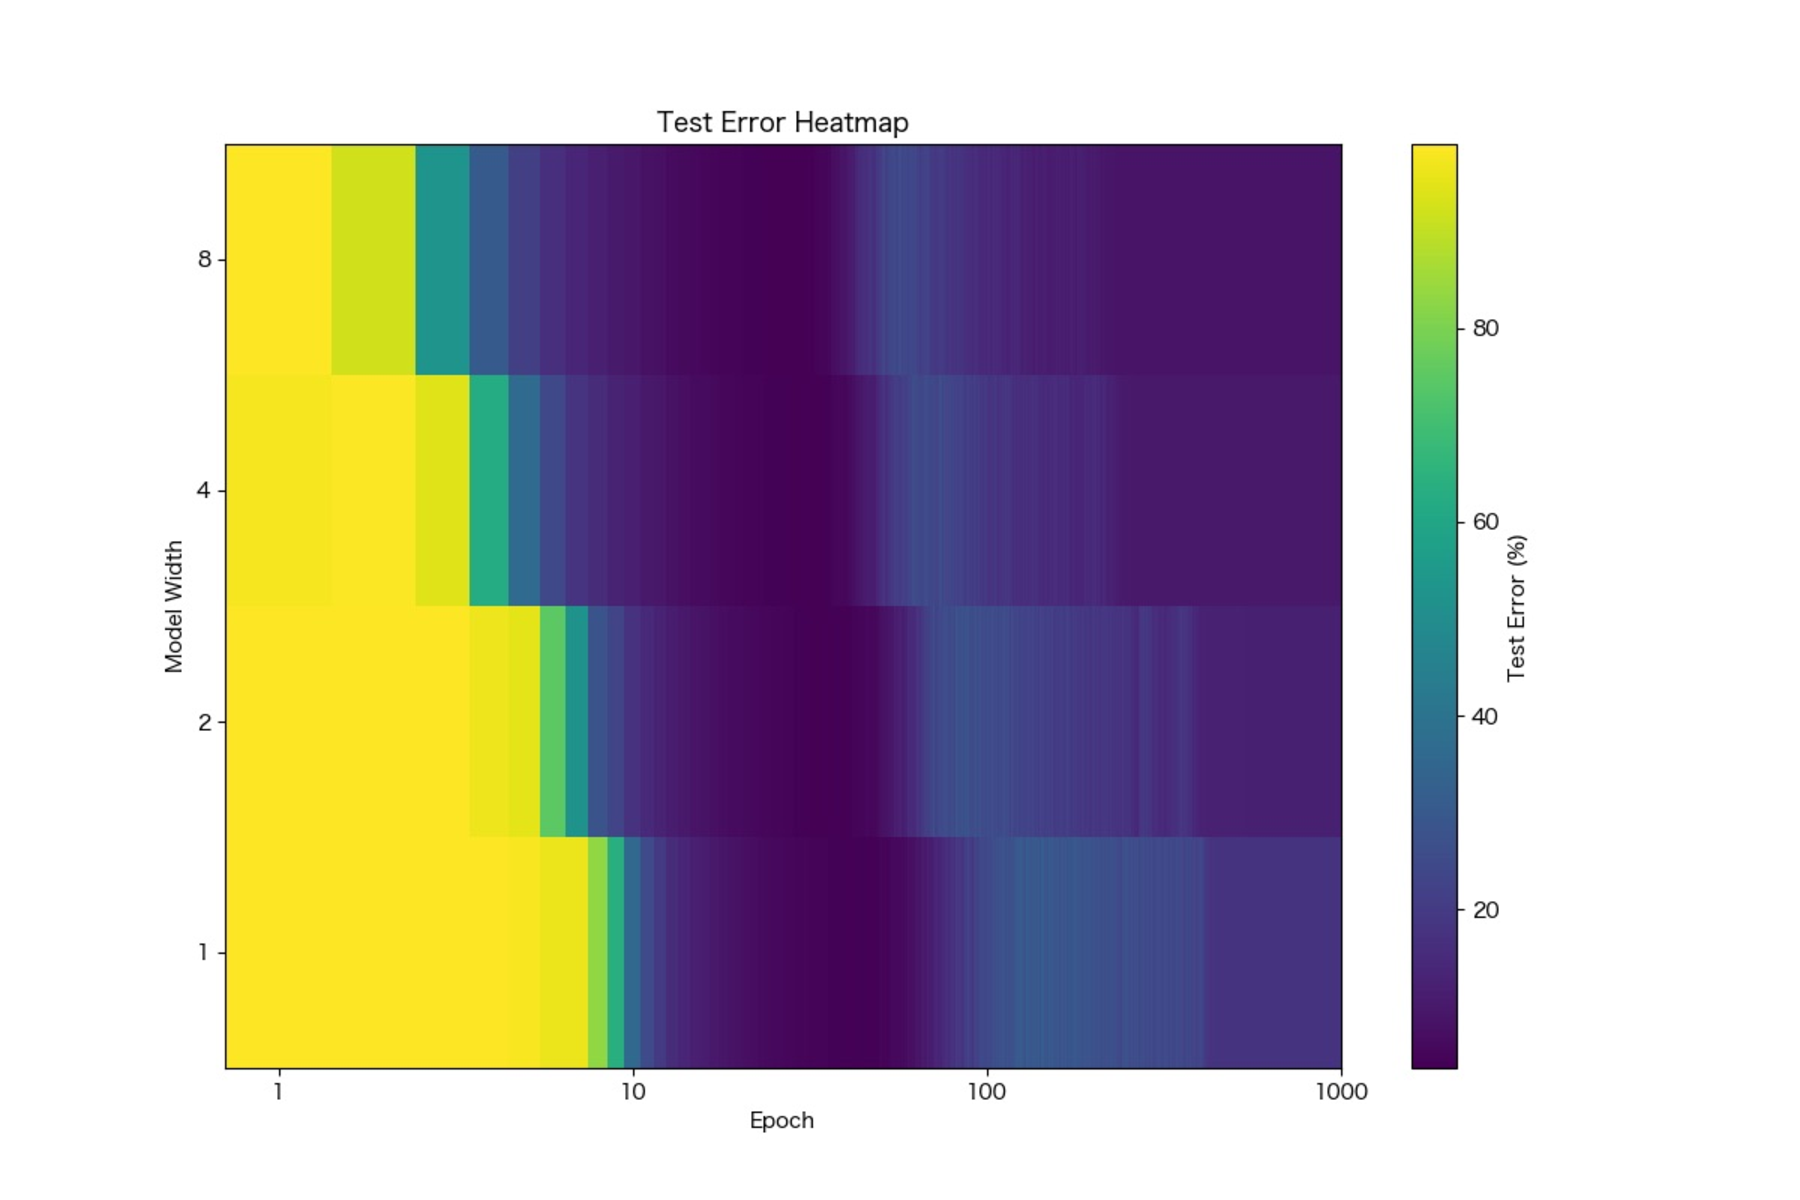
\includegraphics[width=\linewidth]{fig/test_error_heatmap_ln0.2.pdf}
    \caption[$\gamma = 0.2, \sigma^2 = 0$のときのEpochとModel Widthによるテストエラーのヒートマップ]{$\gamma = 0.2, \sigma^2 = 0$のときのEpochとModel Widthによるテストエラーのヒートマップ.
    モデルのチャネル幅が広くなると,過学習が早く発生することが確認できる.エポック軸に見てみると,例えば,8エポック付近では、width wiseで二重降下現象が確認できる}
    \label{fig:modelwidth_heatmap}
\end{figure}
